\section{El Espacio Afín.}\label{Rel:Tema1}


\begin{ejercicio}
    Sea $\cc{A} = \{p\}$ un conjunto con un único elemento. Encuentra qué ha de cumplir un espacio vectorial $V$ para que $\cc{A}$ pueda dotarse de estructura de espacio afín de forma que $V$ sea su espacio de direcciones.\\

    Por la segunda condición de espacio afín, es necesario que exista una biyección $\varphi_p:\cc{A}\to V$. Por tanto, es necesario que $1=|\cc{A}|=|V|$. Por tanto, se tiene que 
    $$\vec{A}=V=\{0\}.$$

    Esto también está demostrado en el ejemplo de la página \pageref{ej:espacio_afin_punto}.
\end{ejercicio}

\begin{ejercicio}
     Sea $V$ un espacio vectorial real. Se considera la siguiente aplicación $\Phi:V\times V \to V$ dada por $\Phi(u, v) = 2u - v$, que denotaremos por $\Phi(u, v) = \vec{uv}$. Estudiar si $\Phi$ induce o no una estructura de espacio afín en $V$.\\

     Consideramos $u,v,w\in V$. Veamos que para dicha aplicación no se cumple la igualdad triangular:
     \begin{equation*}
         \vec{uv} + \vec{vw} = 2u-v+2v-w = 2u+v-w\neq 2u-w=\vec{uw}
     \end{equation*}

     Por tanto, no induce una estructura de espacio afín.
\end{ejercicio}


\begin{ejercicio}
    En el espacio $\cc{P}_2(\bb{R})$ de polinomios de grado $2$ con coeficientes reales,     justifica si los siguientes subconjuntos son subespacios afines de $\cc{P}_2(\bb{R})$. En caso afirmativo, encuentra el subespacio afín paralelo que pasa por el polinomio $p_0(x) = 1 + x^2$.
    \begin{enumerate}
        \item $S = \{a_0^3 + a_1x - x^2 \mid a_0,a_1 \in \bb{R}\}$.
        \begin{equation*}
            S = - x^2 + \{a_0^3 + a_1x \mid a_0,a_1 \in \bb{R}\} \AstIg - x^2 + \{b_0 + a_1x \mid b_0,a_1 \in \bb{R}\} = -x^2 + \cc{L}\{1,x\}
        \end{equation*}
        donde en $(\ast)$ he aplicado que $f:\bb{R}\to \bb{R}$ dada por $f(x)=x^3$ es una biyección, por lo que $\forall~a_0^3\in \bb{R},~\exists_1 b_0\in \bb{R}\mid a_0^3=b_0$.
        
        Por tanto, sí es un plano afín con variedad de direcciones $\cc{L}\{1,x\}$.

        El subespacio afín paralelo que pasa por el polinomio $p_0(x) = 1 + x^2$ es:
        $$S'=p_0 + \cc{L}\{1,x\} = \{1+x^2+b_0 + a_1x\mid b_0,a_1\in \bb{R}\}$$
        
        \item $T = \{p(x) \in P_2(\bb{R}) \mid p(1) = 2, p'(0) = 1\}$.

        Notando $p(x)=a_0+a_1x+a_2x^2$, se tiene que las ecuaciones cartesianas son:
        \begin{align*}
            &p'(0)= 1=a_1\\
            &p(1)=2=a_0+a_1+a_2 \Longrightarrow a_0=1-a_2
        \end{align*}

        Por tanto, $p(x)=1-a_2 + x+a_2x^2=1+x + a_2(x^2-1)$, por lo que:
        $$T=\{1+x+a_2(x^2-1)\mid a_2\in \bb{R}\} = 1+x+\cc{L}\{x^2-1\}$$
        Por tanto, se trata de una recta afín con variedad de direcciones $\cc{L}(x^2-1)$.

        El subespacio afín paralelo que pasa por el polinomio $p_0(x) = 1 + x^2$ es:
        $$T'=p_0 + \cc{L}\{x^2-1\} = \{1+x^2+a_2(x^2-1)\mid a_2\in \bb{R}\}$$
    \end{enumerate}
\end{ejercicio}


\begin{ejercicio}
    En el espacio $\cc{M}_2(\bb{C})$ de matrices cuadradas de orden $2$ con coeficientes complejos, justifica si los siguientes subconjuntos son subespacios afines de $\cc{M}_2(\bb{C})$ y, en caso afirmativo, encuentra el subespacio afín paralelo que pasa por la matriz $\left(\begin{array}{cc}
        1 & i \\
        i & 0
    \end{array}\right)$.
    \begin{enumerate}
        \item $S = \{A \in \cc{M}_2(\bb{C}) \mid tr(A) = 1 + i\}$,

        Empezamos con el primer subconjunto. Tenemos que:
        \begin{equation*}\begin{split}
            S&=\left\{\left(\begin{array}{cc}
                z_1 & z_2 \\
                z_3 & z_4
            \end{array}\right) \in \cc{M}_2(\bb{C}) \mid z_1+z_4=1+i\right\}
            =\\&= \left\{\left(\begin{array}{cc}
                1 & 0 \\
                0 & i
            \end{array}\right)+\left(\begin{array}{cc}
                z_1 & z_2 \\
                z_3 & -z_1
            \end{array}\right) \in \cc{M}_2(\bb{C}) \mid z_1,z_2,z_3\in \bb{C}\right\}
            =\\&= \left(\begin{array}{cc}
                1 & 0 \\
                0 & i
            \end{array}\right) +\left\{\left(\begin{array}{cc}
                z_1 & z_2 \\
                z_3 & -z_1
            \end{array}\right)\mid z_1,z_2,z_3\in \bb{C}\right\}
        \end{split}\end{equation*}
    
        Por tanto, sí es un subespacio afín. El subespacio afín paralelo pedido es:
        $$S'= \left(\begin{array}{cc}
            1 & i \\
            i & 0
        \end{array}\right)+\left\{\left(\begin{array}{cc}
            z_1 & z_2 \\
            z_3 & -z_1
        \end{array}\right)\mid z_1,z_2,z_3\in \bb{C}\right\}$$
        
        \item $T = \{A \in \cc{M}_2(\bb{C}) \mid det(A) = 1\}$.

        Supongamos que sí lo es, y por consiguiente que es un espacio afín. Fijada
        $A=\left(\begin{array}{cc}
                -1 & 0 \\
                0 & -1
            \end{array}\right)\in T$, tenemos la siguiente biyección:
        \Func{\varphi_A}{T}{\vec{T}}{B}{\vec{AB} = B-A}

        Por tanto, tenemos que:
        \begin{equation*}
            \varphi_A \left(\begin{array}{cc}
                0 & i \\
                i & 0
            \end{array}\right) = \left(\begin{array}{cc}
                0 & i \\
                i & 0
            \end{array}\right) - \left(\begin{array}{cc}
                -1 & 0 \\
                0 & -1
            \end{array}\right) = \left(\begin{array}{cc}
                1 & i \\
                i & 1
            \end{array}\right)
        \end{equation*}

        Por tanto, $v=\left(\begin{array}{cc}
                1 & i \\
                i & 1
            \end{array}\right)\in \vec{T}$; y como $\vec{T}$ es un espacio vectorial, tiene que $7v\in \vec{T}$. Como $\varphi_A$ es una biyección, tenemos que $\exists C\in T$ tal que $7v = C-A \Longrightarrow C = 7v + A$. Veamos el valor de $C$:
            \begin{equation*}
                C = 7v+A = \left(\begin{array}{cc}
                7 & 7i \\
                7i & 7
            \end{array}\right) + \left(\begin{array}{cc}
                -1 & 0 \\
                0 & -1
            \end{array}\right) = \left(\begin{array}{cc}
                6 & 7i \\
                7i & 6
            \end{array}\right)
            \end{equation*}

        No obstante, $|C| = 36 - 49i^2 \neq 1$, por lo que $C\notin T$, llegando a una contradicción. Por tanto, no es un subespacio afín.
    \end{enumerate}
\end{ejercicio}


\begin{ejercicio}
    Sean $a, b : \bb{R} \to \bb{R}$ funciones continuas. Definimos los siguientes conjuntos:
    \begin{gather*}
        V = \{ f \in C^1(\bb{R}) \mid f'(x) + a(x)f(x) = 0, ~\forall x \in \bb{R}\},\\
        \cc{A} = \{ f \in C^1(\bb{R}) \mid f'(x) + a(x)f(x) = b(x), ~\forall x \in \bb{R}\},
    \end{gather*}
    donde $C^1(\bb{R})$ es el espacio vectorial real de las funciones de clase $C^1$ sobre los reales. Se pide lo siguiente:
    \begin{enumerate}
        \item Demostrar que $V$ es un espacio vectorial real.

        Como tenemos que $C^1(\bb{R})$ es un espacio vectorial, comprobemos que $V$ es un subespacio vectorial suyo. Sean $f,g\in V$:
        \begin{enumerate}
            \item Veamos si $f+g\in V$:
            \begin{equation*}
                (f+g)'(x) + a(x)(f+g)(x)=f'(x)+g'(x)+a(x)f(x)+a(x)g(x)=0+0=0
            \end{equation*}
            
            \item Veamos si, dado $c\in \bb{R}$, se tiene que $cf\in V$:
            \begin{equation*}
                (cf')(x) + a(x)(cf')(x)=c[f'(x) + a(x)f(x)]=0
            \end{equation*}
        \end{enumerate}
        Por tanto, $V$ es un subespacio vectorial real, y por tanto es un espacio vectorial real.

        
        \item Supongamos sabido que $\cc{A} \neq \emptyset$. Ver si $\cc{A}$ es un espacio afín sobre $V$ cuando, para cada par de funciones $f, g \in A$, definimos $\vec{fg} = g(x)f(x)$.

        En primer lugar, se ha de dar la igualdad triangular:
        \begin{equation*}
            \vec{fg} + \vec{gh} = g(x)f(x)+g(x)h(x) \neq h(x)f(x) = \vec{fh}
        \end{equation*}

        Por tanto, como no se da la igualdad triangular, tenemos que no es un espacio afín sobre $V$. Para que lo fuese, tendría que ser $\vec{fg} = g(x)-f(x)$.
    \end{enumerate}
\end{ejercicio}


\begin{ejercicio}[Producto de espacios afines] Sean $\cc{A}_1$ y $\cc{A}_2$ dos espacios afines sobre espacios vectoriales reales $V_1$ y $V_2$. Se pide lo siguiente:
\begin{enumerate}
    \item Demostrar que el producto cartesiano $\cc{A}_1 \times \cc{A}_2$ es un espacio afín sobre $V_1 \times V_2$ cuando definimos:
    \begin{equation*}
        \vec{(p_1, p_2)(q_1, q_2)} = (\vec{p_1q_1}, \vec{p_2q_2}).
    \end{equation*}

    Veamos que $\vec{\cdot}$ cumple las dos condiciones necesarias para que sea un espacio afín:
    \begin{enumerate}
        \item Comprobamos la igualdad triangular:
        \begin{equation*}\begin{split}
            \vec{(p_1, p_2)(q_1, q_2)} +&\vec{(q_1, q_2)(t_1, t_2)}
            = (\vec{p_1q_1}, \vec{p_2q_2}) + (\vec{q_1t_1}, \vec{q_2t_2}) =\\
            &= (\vec{p_1q_1}+\vec{q_1t_1}, \vec{p_2q_2}+\vec{q_2t_2})
            \AstIg (\vec{p_1t_1}, \vec{p_2t_2}) = \vec{(p_1, p_2)(t_1, t_2)}
        \end{split}\end{equation*}
        donde en $(\ast)$ he aplicado que $V_1,V_2$ son, en concreto, espacios afines.

        \item Comprobamos ahora que, fijado $p_1\in \cc{A}_1,p_2\in \cc{A}_2$, se tiene que la siguiente aplicación es biyectiva:
        \Func{\varphi_{p_1,p_2}}{\cc{A}_1\times \cc{A}_2}{V_1\times V_2}{(q_1,q_2)}{\vec{(p_1, p_2)(q_1, q_2)}}

        Vemos ahora que, para $i=1,2$, la siguiente aplicación es biyectiva:
        \Func{\varphi_{p_i}}{\cc{A}_i}{V_i}{q_i}{\vec{p_iq_i}}
        
        Tenemos además lo siguiente:
        $$\vec{(p_1, p_2)(q_1, q_2)}=(q_1,q_2) - (p_1,p_2)=(q_1-p_1,q_2-p_2) = \left(\vec{p_1q_1},\vec{p_2q_2}\right)$$

        Por tanto, tenemos que la función queda como:
        \Func{\varphi_{p_1,p_2}}{\cc{A}_1\times \cc{A}_2}{V_1\times V_2}{(q_1,q_2)}{\left(\vec{p_1q_1},\vec{p_2q_2}\right)}

        Esta es claramente biyectiva, por serlo en cada una de las variables.
    \end{enumerate}
    
    \item Supongamos que $\dim(\cc{A}_1) = m$ y $\dim(\cc{A}_2) = n$. Sea $\cc{R}_i = \{ o_i, \cc{B}_i\}$ un sistema de referencia en $\cc{A}_i,~i = 1, 2$. Pongamos $\cc{B}_1 = \{u_1, \dots , u_m\}$ y $\cc{B}_2 = {v_1, \dots , v_n}$. Demostrar que el par $\cc{R}_1 \times \cc{R}_2 = \{(o_1, o_2), \cc{B}_1 \times \cc{B}_2\}$, donde
    \begin{equation*}
        \cc{B}_1 \times \cc{B}_2 = \{ (u_1, 0), \dots ,(u_m, 0),(0, v_1), \dots ,(0, v_n)\},
    \end{equation*}
    es un sistema de referencia en $\cc{A}_1 \times \cc{A}_2$. A partir de aquí concluir el siguiente resultado: $\dim(\cc{A}_1 \times \cc{A}_2) = n + m$.\\

    Para ver que es un sistema de referencia, hemos de ver dos aspectos. En primer lugar, es necesario que el origen $(o_1,o_2)\in \cc{A}_1\times \cc{A}_2$, lo cual es evidente ya que $o_i\in \cc{A}_i$ para $i=1,2$. Veamos ahora que $\cc{B}_1\times \cc{B}_2$ es una base:
    \begin{equation*}\begin{split}
        (0,0)&=a_1(u_1,0)+ \dots a_m(u_m,0) + b_1(0,v_1) + \dots b_n(0,v_n) =\\
        &= (a_1u_1+\dots + a_mu_m, b_1v_1 + \dots b_nv_n) \qquad a_i,b_i\in \bb{R}
    \end{split}\end{equation*}
    Por tanto, como ambas son una base en el respectivo espacio vectorial, tenemos que $a_i,b_j= 0,~\forall i,j$, es decir, $\cc{B}_1\times \cc{B}_2$ es una base de ${V}_1\times {V}_2$.
    
    Por tanto, tenemos que $\cc{R}_1\times \cc{R}_2$ es un sistema de referencia. Además, como la base asociada tiene $n+m$ vectores linealmente independientes, implica que $\dim \vec{\cc{A}_1\times \cc{A}_2}=n+m$ y, por tanto, $\dim {\cc{A}_1\times \cc{A}_2}=n+m$.
    

    \item Sea $(p_1, p_2) \in \cc{A}_1 \times \cc{A}_2$. ¿Cómo se relacionan las coordenadas de $(p_1, p_2)$ en $\cc{R}_1 \times \cc{R}_2$ con las coordenadas de $p_i$ en $\cc{R}_i,~i = 1, 2$?\\

    Sea ${p_1}_{\cc{R}_1}=(a_1,\dots,a_m)$ y ${p_2}_{\cc{R}_2}=(b_1,\dots,b_n)$. Entonces, por definición de coordenadas tenemos que $p_1=o_1+a_1u_1+\dots+a_mu_m$. Análogamente, tenemos que $p_2=o_2+b_1v_1+\dots+b_n v_n$. Por tanto, tenemos que:
    \begin{equation*}\begin{split}
        (p_1,p_2) &=(o_1+a_1u_1+\dots + a_mu_m, o_2 + b_1v_1 + \dots b_nv_n) =\\
        &= (o_1,o_2) + a_1(u_1,0)+ \dots a_m(u_m,0) + b_1(0,v_1) + \dots b_n(0,v_n)
    \end{split}\end{equation*}

    Por tanto, tenemos que ${(p_1,p_2)}_{\cc{R}_1\times \cc{R}_2}=(a_1,\dots, a_m,b_1,\dots,b_n)$. Como podemos ver, se concatenan las coordenadas.
\end{enumerate}
\end{ejercicio}



\begin{ejercicio}
    En $\bb{R}^3$ consideramos el conjunto $\cc{R} = \{a_0, a_1, a_2, a_3\}$ formado por los puntos:
    \begin{equation*}
        a_0 = (1, 2, 1),\qquad  a_1 = (2, 1, 0),\qquad a_2 = (0, 1, 0),\qquad a_3 = (1,-1, 2).
    \end{equation*}
    Demostrar que $\cc{R}$ es un sistema de referencia afín de $\bb{R}^3$. Calcular las coordenadas afines del punto $p = (0, 0, 0)$ en este sistema de referencia.\\

    Consideramos los siguientes vectores:
    \begin{equation*}
        \vec{a_0a_1} = (1,-1,-1) \qquad \vec{a_0a_2} = (-1,-1,-1) \qquad \vec{a_0a_3} = (0,-3,1)
    \end{equation*}

    Para ver que esos tres vectores son linealmente independientes, comprobamos que el siguiente determinante no es nulo:
    \begin{equation*}
        \left|\begin{array}{ccc}
            1 & -1 & 0 \\
            -1 & -1 & -3 \\
            -1& -1 & 1
        \end{array}\right| = \left|\begin{array}{ccc}
            1 & -1 & 0 \\
            -1 & -1 & -3 \\
            0& 0 & 4
        \end{array}\right| = 4\cdot (-1 -1)=-8\neq 0
    \end{equation*}

    Por tanto, tenemos que esos tres vectores son linealmente independientes, por lo que los puntos de $\cc{R}$ son afínmente independientes, teniendo entonces efectivamente que forman un sistema de referencia, con origen $a_0$ y base asociada la siguiente: $\cc{B}=\{\vec{a_0a_1},\vec{a_0a_2},\vec{a_0a_3}\}$.\\

    Veamos ahora las coordenadas de $p$ en $\cc{R}$:
    \begin{equation*}\begin{split}
        \vec{a_0(0,0,0)} &= (-1,-2,-1) = b_1\vec{a_0a_1} + b_2\vec{a_0a_2} + b_3\vec{a_0a_3}= \\
        & = b_1(1,-1,-1) +b_2(-1,-1,-1) + b_3(0,-3,1) =\\
        &= (b_1-b_2, -b_1-b_2-3b_3, -b_1-b_2+b_3)
    \end{split}\end{equation*}

    Por tanto, quedan las siguientes ecuaciones:
    \begin{equation*}
        \left\{
        \begin{array}{rcl}
            b_1-b_2 &=& -1  \\
            -b_1-b_2-3b_3 &=& -2 \\
            -b_1-b_2+b_3 &=& -1
        \end{array}
        \right\} \Longrightarrow \begin{array}{rcl}
            b_1=\nicefrac{1}{8}  \\
            b_2 = \nicefrac{9}{8} \\
            b_3= \nicefrac{1}{4}
        \end{array}
    \end{equation*}
    Por tanto, tenemos que $p_{\cc{R}}=\displaystyle \left(\frac{1}{8},\frac{9}{8},\frac{1}{4}\right)$.
\end{ejercicio}

\begin{ejercicio}
    Consideremos el punto $p = (1,2,3) \in \bb{R}^3$. Encontrar un sistema de referencia $\cc{R}$ de $\bb{R}^3$ de forma que $p_{\cc{R}} = (1,0, 2)$. ¿Es el sistema de referencia anterior único?

    Sea $p_0\in \bb{R}^3$ y una base $\cc{B}=\{v_1,v_2,v_3\}$. Buscamos un sistema de referencia $\cc{R}=\{p_0,\cc{B}\}$ tal que $p_{\cc{R}} = (1,0, 2)$. Tenemos que la fórmula de cambio de sistema de referencia es:
    \begin{equation*}
        p_{\cc{R}} = (0)_{\cc{R}} + M(\cc{B}_u,\cc{B})\cdot p_{\cc{R}_0}
    \end{equation*}

    Esto es:
    \begin{equation*}
        \left(\begin{array}{c}
            1 \\ 0 \\ 2
        \end{array}\right) = 
        \left(\begin{array}{c}
            x \\ y \\ z
        \end{array}\right) + \left(\begin{array}{ccc}
            a_1 & b_1 & c_1 \\
            a_2 & b_2 & c_2 \\
            a_3 & b_3 & c_3 \\
        \end{array}\right)
        \left(\begin{array}{c}
            1 \\ 2 \\ 3
        \end{array}\right)
    \end{equation*}

    Equivalentemente, 
    \begin{equation*}
        \left(\begin{array}{c}
            1 \\\hline 1 \\ 0 \\ 2
        \end{array}\right) = \left(\begin{array}{c|ccc}
            1 & 0 & 0 & 0 \\ \hline
            x & a_1 & b_1 & c_1 \\
            y & a_2 & b_2 & c_2 \\
            z & a_3 & b_3 & c_3 \\
        \end{array}\right)
        \left(\begin{array}{c}
            1 \\\hline 1 \\ 2 \\ 3
        \end{array}\right)
    \end{equation*}


    Por tanto, tengo 12 incógnitas y 3 ecuaciones linealmente independientes. Por tanto, el sistema de referencia no es único. Una posible solución es usar $\cc{B}=\cc{B}_u$, y calcular el nuevo origen:
    \begin{equation*}
        \left(\begin{array}{c}
            1 \\ 0 \\ 2
        \end{array}\right) = 
        \left(\begin{array}{c}
            x \\ y \\ z
        \end{array}\right) + Id_3
        \left(\begin{array}{c}
            1 \\ 2 \\ 3
        \end{array}\right)
    \end{equation*}
    De forma que obtenemos $x=0, y=-2, z=-1$. El sistema de referencia pedido es:
    \begin{equation*}
        \cc{R}=\{(0, -2, -1),\cc{B}_u\}
    \end{equation*}

    Otra posible solución es usar como matriz de cambio de base, $-Id_3$. De esta forma, si $\cc{B}_u=\{e_1,e_2,e_3\}$, tenemos que $\cc{B}=\{-e_1,-e_2,-e_3\}$. Así, se tiene que el nuevo origen tiene de coordenadas $(2, 2, 5)$, por lo que otro posible sistema de coordenadas que cumpla lo pedido es:
    \begin{equation*}
        \cc{R}=\{(2,2,5),\{-e_2,-e_2,-e_3\}\}
    \end{equation*}
\end{ejercicio}


\begin{ejercicio}
    En $\bb{R}^2$ consideremos los conjuntos $\cc{R} = \{(1, 1),(1, -1),(2, 1)\}$ y $\cc{R}' = \{(1, 2),(2, 2),(2, 0)\}$.
    \begin{enumerate}
        \item Comprueba que son sistemas de referencia de $\bb{R}^2$.

        Para que $\cc{R}$ sea un sistema de referencia, es necesario que $\{\vec{(1,1)(1,-1)}, \vec{(1,1)(2,1)}\}$ sea una base:
        \begin{equation*}
            \cc{B}=\{\vec{(1,1)(1,-1)}, \vec{(1,1)(2,1)}\}
            = \{{(0,-2)}, {(1,0)}\}
        \end{equation*}
        Como $\cc{B}$ es una base, tenemos que $\cc{R}$ es un sistema de referencia.\\
    
        Para $\cc{R}'$, es necesario que $\{\vec{(1,2)(2,2)}, \vec{(1,2)(2,0)}\}$ sea una base:
        \begin{equation*}
            \cc{B}'=\{\vec{(1,2)(2,2)}, \vec{(1,2)(2,0)}\}
            = \{{(1,0)}, {(1,-2)}\}
        \end{equation*}
        Como $\cc{B}'$ es una base, tenemos que $\cc{R}'$ es un sistema de referencia.
        
        \item  Calcula las ecuaciones que representan el cambio de sistema de referencia de $\cc{R}$ a $\cc{R}'$ y las de $\cc{R}'$ a $\cc{R}$.

        Dado $p\in \cc{A}$, sean las coordenadas en ambos sistemas de referencia los siguientes:
        \begin{equation*}
            p_{\cc{R}}=(x,y)\hspace{1cm}
            p_{\cc{R}'}=(s,t)
        \end{equation*}

        Entonces, por definición de sistema de referencia, tenemos que:
        \begin{equation*}
            \left\{
            \begin{array}{lllll}
                p&=&(1,1) +x(0,-2) + y(1,0) &=& (1+y, 1-2x) \\
                p&=&(1,2) +s(1,0) + t(1,-2) &=& (1+s+t, 2-2t)
            \end{array}
            \right.
        \end{equation*}

        Igualando componentes, tenemos que:
        \begin{equation*}
            \left\{
            \begin{array}{lll}
                1+y&=&1+s+t\\
                1-2x&=&2-2t
            \end{array}
            \right.
        \end{equation*}

        Por tanto, tenemos que el cambio de variable de $\cc{R}'$ a $\cc{R}$ es:
        \begin{equation*}
            \left\{
            \begin{array}{lll}
                x & = & \frac{1}{2}(-1+2t) \\
                y & = & s+t
            \end{array}
            \right.
        \end{equation*}

        Matricialmente, tenemos que el cambio de variable de $\cc{R}'$ a $\cc{R}$ es:
        \begin{equation*}
            \left(\begin{array}{c}
                x \\ y
            \end{array}\right)
            = 
            \left(\begin{array}{c}
                \nicefrac{-1}{2}\\ 0
            \end{array}\right)
            +
            \left(\begin{array}{ccc}
                0 & 1 \\
                1 & 1
            \end{array}\right)
            \left(\begin{array}{c}
                s \\ t
            \end{array}\right)
        \end{equation*}

        El cambio de variable de $\cc{R}$ a $\cc{R}'$ es:
        \begin{equation*}
            \left\{
            \begin{array}{lll}
                s & = & -\frac{1}{2}-x+y \\
                t & = & \frac{1}{2}(1+2x)
            \end{array}
            \right.
        \end{equation*}
        
        
        \item Calcula las coordenadas del punto $(0, 1)$ en los sistemas de referencia $\cc{R}$ y $\cc{R}'$.

        Sea $(0,1)_{\cc{R}}=(x,y)$. Entonces, tenemos que:
        \begin{equation*}
            (0,1)=(1,1) +x(0,-2) +y(1,0) = (1+y, 1-2x)
        \end{equation*}
        Por tanto, $x=0,y=-1$. Es decir, $(0,1)_{\cc{R}}=(0,-1)$.

        Aplicando el cambio de sistema de referencia de $\cc{R}$ a $\cc{R}'$, tenemos las coordenadas que nos faltan: $(0,1)_{\cc{R}'}=\left(-\frac{3}{2},\frac{1}{2}\right)$
    \end{enumerate}
\end{ejercicio}

\begin{ejercicio}
    Sea $C = \{(x, y) \in \bb{R}^2 \mid x^2 + y^2 = 1\}$ la circunferencia unidad de $\bb{R}^2$ y el sistema de referencia $\cc{R} = \{(1, -1),(1, 0),(2, 0)\}$ de $\bb{R}^2$. Calcula la ecuación de $C$ en el sistema de referencia $\cc{R}$.\\

    Sea $p=(x,y)\in \bb{R}^2$, y consideramos sus coordenadas en $\cc{R}$, $p_{\cc{R}}=(s,t)$. Entonces,
    \begin{equation*}
        p=(x,y) = (1,-1) + s\vec{(1,-1)(1,0)} +t\vec{(1,-1)(2,0)}
        = (1,-1) + s(0,1) +t(1,1)
    \end{equation*}
    
    Por tanto,
    \begin{equation*}
        \left\{
        \begin{array}{lll}
            x & = & 1+t \\
            y & = & -1+s+t
        \end{array}
        \right.
    \end{equation*}

    Tenemos por tanto que:
    \begin{equation*}
        p\in C\Longleftrightarrow x^2+y^2=1 \Longleftrightarrow
        (1+t)^2 + (-1+s+t)^2=1
    \end{equation*}

    Es decir,
    \begin{equation*}
        C=\{(s,t)_{\cc{R}}\in \bb{R}^2\mid (1+t)^2 + (-1+s+t)^2=1\}
    \end{equation*}
\end{ejercicio}


\begin{ejercicio}
    En un plano afín $\cc{A}$ se consideran dos puntos $a_1, a_2\in \cc{A}$ y una base $\cc{B} = \{e_1, e_2\}$. Sea también $\cc{B}'=\{e_1 + e_2, e_1 - e_2\}$.
    Considérense los sistemas de referencia $\cc{R}=\{a_1,\cc{B}\}$ y $\cc{R}'=\{a_2,\cc{B}'\}$. Si el vector $(\vec{a_1a_2})_\cc{B} = (1, 1)$, calcula:
    \begin{enumerate}
        \item Las ecuaciones de cambio de sistema de referencia de $\cc{R}$ a $\cc{R}'$ y de $\cc{R}'$ a $\cc{R}$.

        Como $(\vec{a_1a_2})_\cc{B} = (1, 1)$, tenemos que $\vec{a_1a_2}=a_2-a_1 = e_1+e_2$. Por tanto, tenemos que las coordenadas de $a_1,a_2$ en respectivos sistemas de referencia son::
        \begin{gather*}
            a_2 = a_1 + e_1+e_2 \Longrightarrow (a_2)_{\cc{R}} = (1,1) \\
            a_1 = a_2 - e_1-e_2 \Longrightarrow (a_1)_{\cc{R}'} = (-1,0)
        \end{gather*}

        Además, las matrices de cambio de base son:
        \begin{equation*}
            M(\cc{B}',\cc{B}) = \left(\begin{array}{cc}
                1 & 1 \\
                1 & -1
            \end{array}\right)
            \hspace{1cm}
            M(\cc{B},\cc{B}') =\frac{1}{2}\left(\begin{array}{cc}
                1 & 1 \\
                1 & -1
            \end{array}\right)
        \end{equation*}

        Por tanto, dado $p\in \cc{A}$, con $p_\cc{R}=(x,y)$, $p_{\cc{R}'}=(s,t)$, tenemos que las ecuaciones de cambio de sistema de referencia de $\cc{R}'$ a $\cc{R}$ son:
        \begin{equation*}
            \left(\begin{array}{c}
                x \\ y
            \end{array}\right)
            = 
            \left(\begin{array}{c}
                1\\ 1
            \end{array}\right)
            +
            \left(\begin{array}{ccc}
                1 & 1 \\
                1 & -1
            \end{array}\right)
            \left(\begin{array}{c}
                s \\ t
            \end{array}\right)
        \end{equation*}

        Las ecuaciones de cambio de sistema de referencia de $\cc{R}$ a $\cc{R}'$ son:
        \begin{equation*}
            \left(\begin{array}{c}
                s \\ t
            \end{array}\right)
            = 
            \left(\begin{array}{c}
                -1\\ 0
            \end{array}\right)
            +
            \frac{1}{2}\left(\begin{array}{ccc}
                1 & 1 \\
                1 & -1
            \end{array}\right)
            \left(\begin{array}{c}
                x \\ y
            \end{array}\right)
        \end{equation*}
        
        \item Las coordenadas de $a_1$ y $a_2$ en cada sistema de referencia.

        Como hemos visto antes, tenemos que $(a_2)_{\cc{R}} = (1,1)$, $(a_1)_{\cc{R}'} = (-1,0)$. Además, tenemos que $a_2=a_2+0$ y $a_1=a_1+0$, por lo que $(a_2)_{\cc{R}'} = (0,0)$, $(a_1)_{\cc{R}} = (0,0)$. Es decir,
        \begin{equation*}\begin{split}
            (a_1)_{\cc{R}} = (0,0) &\hspace{1cm} (a_2)_{\cc{R}} = (1,1) \\
            (a_1)_{\cc{R}'} = (-1,0) &\hspace{1cm} (a_2)_{\cc{R}'} = (0,0) \\
        \end{split}\end{equation*}
        
        \item El valor de $t \in \bb{R}$ para que el punto $p$ de coordenadas $p_\cc{R} = (t, 2)$ esté alineado con $a_1$ y $a_2$. ¿Cuáles son las coordenadas de este punto respecto de $\cc{R}'$?

        Tenemos que $p_{\cc{R}}-(a_1)_{\cc{R}}=(t,2)=(\vec{a_1p})_{\cc{B}}$. Además, $(\vec{a_1a_2})_{\cc{B}}=(1,1)$. Para que los tres puntos estén alineados, ambos vectores han de ser proporcionales, por lo que $t=2$.

        Usando las ecuaciones de cambio de sistema de referencia de $\cc{R}$ a $\cc{R}'$, tenemos que $p_{\cc{R}'}=(1,0)$.

        \begin{figure}[H]
            \centering
            \begin{tikzpicture}
            % Ejes
            \draw[-stealth] (-1,0) -- (3,0) node[right] {$x$};
            \draw[-stealth] (0,-1) -- (0,3) node[above] {$y$};
            
            % Puntos
            \fill (0,0) circle (1.5pt) node[below left] {$(a_1)_{\cc{R}} = (0,0)$};
            \fill (1,2) circle (1.5pt) node[above right] {$p_{\cc{R}}=(t,2)$};
            \fill (1,1) circle (1.5pt) node[above right] {$(a_2)_{\cc{R}} = (1,1)$};
        
            % Vector de A a B
            \draw[-stealth, dashed] (0,0) -- (1,1);
        \end{tikzpicture}
        \end{figure}
    \end{enumerate}
\end{ejercicio}


\begin{ejercicio}
     Sea $\cc{R}$ un sistema de referencia de un espacio afín tridimensional $\cc{A}$. Demuestra que $\cc{R}' = \{a_0, a_1, a_2, a_3\}$ con
     $$(a_{0})_{\cc{R}} = (1, 0, 1),\quad (a_{1})_{\cc{R}} = (-1, 0, 1),\quad (a_{2})_{\cc{R}} = (1, 1, 1),\quad (a_{3})_{\cc{R}} = (2, 1, 2),$$
     es otro sistema de referencia. ¿Cuáles son las coordenadas del origen de $\cc{R}$ en el sistema de referencia $\cc{R}'$?\\

     Notemos $\cc{R} = \{b_0, b_1, b_2, b_3\} = \{b_0, \cc{B}\}$, $\cc{R}'=\{a_0,\cc{B'}\}$.

     Veamos los vectores de la base asociada a $\cc{R}'$, para saber si sus vectores son linealmente independientes.Tenemos que:
     \begin{equation*}\begin{split}
         (a_{1})_{\cc{R}}-(a_{0})_{\cc{R}}&=(-2,0,0)=(\vec{a_0a_1})_{\cc{B}} \\
         (a_{2})_{\cc{R}}-(a_{0})_{\cc{R}}&=(0,1,0)=(\vec{a_0a_2})_{\cc{B}} \\
         (a_{3})_{\cc{R}}-(a_{0})_{\cc{R}}&=(1,1,1)=(\vec{a_0a_3})_{\cc{B}}
     \end{split}\end{equation*}

     Como esos tres vectores son linealmente independientes, tenemos que $\cc{R}'$ es un sistema de referencia. La ecuación de cambio de sistema de referencia de $\cc{R}$ a $\cc{R}'$ es:
     \begin{equation*}\begin{split}
         p_{\cc{R}'} &= (b_0)_{\cc{R}'} + M(\cc{B},\cc{B}')p_{\cc{R}}
         = (b_0)_{\cc{R}'} + M(\cc{B}',\cc{B})^{-1}p_{\cc{R}}
         =\\&= (b_0)_{\cc{R}'} + \left(
            \begin{array}{ccc}
                -2 & 0 & 1 \\
                0 & 1 & 1 \\
                0 & 0 & 1
            \end{array}
         \right)^{-1}p_{\cc{R}}
         = (b_0)_{\cc{R}'} + \left(
            \begin{array}{ccc}
                \nicefrac{-1}{2} & 0 & \nicefrac{1}{2} \\
                0 & 1 & -1 \\
                0 & 0 & 1
            \end{array}
         \right)p_{\cc{R}}
     \end{split}\end{equation*}

     Usando $p=a_0$ (podríamos usar cualquier otro punto), tenemos:
     \begin{equation*}\begin{split}
         \left(\begin{array}{c}
             0 \\ 0 \\ 0
         \end{array}\right) &= (b_0)_{\cc{R}'} + \left(
            \begin{array}{ccc}
                \nicefrac{-1}{2} & 0 & \nicefrac{1}{2} \\
                0 & 1 & -1 \\
                0 & 0 & 1
            \end{array}
         \right)\left(\begin{array}{c}
             1 \\ 0 \\ 1
         \end{array}\right)
         = (b_0)_{\cc{R}'} + \left(\begin{array}{c}
             0 \\ -1 \\ 1
         \end{array}\right)
     \end{split}\end{equation*}

     Por tanto, $(b_0)_{\cc{R}'} = -(0, -1, 1) = (0,1,-1)$.
\end{ejercicio}

\begin{ejercicio}
    Demuestra que toda recta afín de $\bb{R}^3$ es la intersección de dos planos afines. ¿Es cierta esta afirmación en $\bb{R}^n$, para cualquier $n \geq 4$?\\

    Sea la recta afín $r=p+\cc{L}\{u\}$. Extendemos la base de $\vec{r}$ a una base del espacio; es decir, $\bb{R}^3=\cc{L}\{u,v,w\}$, con los tres vectores linealmente independientes. Sean ahora los siguientes planos:
    \begin{equation*}
        \pi_1 = p+\cc{L}\{u,v\} \qquad \pi_2 = p+\cc{L}\{u,w\}
    \end{equation*}

    Entonces $\pi_1\cap \pi_2 =  p + \cc{L}\{u\}$, por lo que se tiene.\\

    Este razonamiento también es válido para $\bb{R}^n$, con $n\geq 4$. Esto se debe a que, al extender a una base del espacio, tomamos $\bb{R}^n=\cc{L}\{u,v,w,e_4,\dots,e_n\}$, donde tan solo usaremos los tres primeros vectores para construir los dos planos descritos anteriormente.
\end{ejercicio}

\begin{ejercicio}
    Sean $\cc{R}$ un sistema de referencia de un espacio afín $\cc{A}$ y $S \subset \cc{A}$ un subespacio afín. Si $S$ está definido por las ecuaciones
    \begin{equation*}
        \left\{\begin{array}{c}
            a_{11}x_1+a_{12}x_2 + \dots + a_{1n}x_n=b_1, \\
            \dots \\
            a_{m1}x_1+a_{m2}x_2 + \dots + a_{mn}x_n=b_m, \\
        \end{array}\right.
    \end{equation*}
    en el sistema de referencia $\cc{R}$, entonces demuestra que las ecuaciones de $\vec{S}$ vienen dadas por
    \begin{equation*}
        \left\{\begin{array}{c}
            a_{11}x_1+a_{12}x_2 + \dots + a_{1n}x_n=0, \\
            \dots \\
            a_{m1}x_1+a_{m2}x_2 + \dots + a_{mn}x_n=0, \\
        \end{array}\right.
    \end{equation*}
    en coordenadas respecto de la base asociada a $\cc{R}$.\\

    Sea $\cc{B}$ la base asociada a $\cc{R}$. 
    Por ser $S$ un espacio afín, tenemos que fijado un punto $p\in S$, existe una biyección $\varphi_p:S\to \vec{S}$ dada por $\varphi_p(q)=\vec{pq}$. Por tanto, dado $v\in \vec{S}$, se tiene que $\exists q\in S$ tal que $v=\vec{pq}$. Buscamos demostrar que, si $v_{\cc{B}}=(\vec{pq})_{\cc{B}}=(x_1,\dots,x_n)$, entonces cumple las ecuaciones cartesianas descritas.
    
    Tenemos que $(x_1,\dots,x_n)=(\vec{pq})_{\cc{B}}=q_{\cc{R}}-p_{\cc{R}}$. Sean las coordenadas de $p,q\in S$ las siguientes: $q_{\cc{R}}=(c_1,\dots,c_n)$, $p_{\cc{R}}=(d_1,\dots,d_1)$. Entonces, como ambos puntos pertenecen a $S$, sus coordenadas en $\cc{R}$ cumplen las ecuaciones cartesianas dadas:
    \begin{equation*}
        q\in S,~q_{\cc{R}}=(c_1,\dots,c_n)\Longrightarrow \left\{\begin{array}{c}
            a_{11}c_1+a_{12}c_2 + \dots + a_{1n}c_n=b_1, \\
            \dots \\
            a_{m1}c_1+a_{m2}c_2 + \dots + a_{mn}c_n=b_m, \\
        \end{array}\right.
    \end{equation*}
    \begin{equation*}
        p\in S,~p_{\cc{R}}=(d_1,\dots,d_n)\Longrightarrow\left\{\begin{array}{c}
            a_{11}d_1+a_{12}d_2 + \dots + a_{1n}d_n=b_1, \\
            \dots \\
            a_{m1}d_1+a_{m2}d_2 + \dots + a_{mn}d_n=b_m, \\
        \end{array}\right.
    \end{equation*}

    Igualando los valores de $b_i$ para todo $i\in \{1,\dots m\}$, tenemos:
    \begin{equation*}
        \left\{\begin{array}{c}
            a_{11}c_1+a_{12}c_2 + \dots + a_{1n}c_n=a_{11}d_1+a_{12}d_2 + \dots + a_{1n}d_n, \\
            \dots \\
            a_{m1}c_1+a_{m2}c_2 + \dots + a_{mn}c_n=a_{m1}d_1+a_{m2}d_2 + \dots + a_{mn}d_n, \\
        \end{array}\right.
    \end{equation*}

    Llevando todo al término de la izquierda y sacando factor común, tenemos:
    \begin{equation*}
        \left\{\begin{array}{c}
            a_{11}(c_1-d_1)+a_{12}(c_2-d_2) + \dots + a_{1n}(c_n-d_n)=0, \\
            \dots \\
            a_{m1}(c_1-d_1)+a_{m2}(c_2-d_2) + \dots + a_{mn}(c_n-d_n)=0, \\
        \end{array}\right.
    \end{equation*}
    
    Precisamente, tenemos que $$(x_1,\dots,x_n)=(\vec{pq})_{\cc{B}}=q_{\cc{R}}-p_{\cc{R}}=(c_1-d_1,\dots, c_n-d_n)$$
    Por tanto, se tiene demostrado que las ecuaciones dadas son las ecuaciones cartesianas de $\vec{S}$ respecto a $\cc{B}$.
\end{ejercicio}


\begin{ejercicio}
    Sea $\cc{A}$ un espacio afín con sistema de referencia $\cc{R}$ y $S$ el conjunto de puntos $p \in \cc{A}$ tales que $p_\cc{R} = (x_1, \dots, x_n)$ es solución del sistema de ecuaciones lineales
    \begin{equation*}
        \left\{\begin{array}{c}
            a_{11}x_1+a_{12}x_2 + \dots + a_{1n}x_n=b_1, \\
            \dots \\
            a_{m1}x_1+a_{m2}x_2 + \dots + a_{mn}x_n=b_m, \\
        \end{array}\right.
    \end{equation*}
    Demuestra que $S$ es un subespacio afín de $\cc{A}$.

    Sea $\cc{B}$ la base asociada a $\cc{R}$. Supongamos $S\neq 0$ (no se puede probar por falta de información en el enunciado). Sea por tanto $p\in S$ con $p_{\cc{R}}=(d_1,\dots,d_n)$, que cumple las ecuaciones dadas. Consideramos $q\in S$. Entonces, tenemos que: $$q_{\cc{R}}-p_{\cc{R}}=(\vec{pq})_{\cc{B}} \in \vec{\cc{A}}$$
    
    
    Sean las coordenadas de $\vec{pq}$ las siguientes: $$(\vec{pq})_{\cc{B}}=(x'_1,\dots,x'_n):=(x_1,\dots,x_n)-(d_1,\dots,d_n)$$
    
    
    Veamos ahora que  $a_{i1}x_1'+a_{i2}x_2' + \dots + a_{in}x_n'=0$ para todo $i\in \{0,\dots,m\}$:
    \begin{equation*}
        \begin{split}
            a_{i1}&x_1'+a_{i2}x_2' + \dots + a_{in}x_n'=\\
            &= a_{i1}(x_1-d_1)+a_{i2}(x_2-d_2) + \dots + a_{in}(x_n-d_n) =\\
            &= b_i-b_i=0
        \end{split}
    \end{equation*}
    
    Por tanto, tenemos que:
    \begin{equation*}
        \begin{split}
            S &= \left\{
            (x_1,\dots,x_n) \left|
            \begin{array}{c}
                a_{11}x_1+a_{12}x_2 + \dots + a_{1n}x_n=b_1, \\
                \dots \\
                a_{m1}x_1+a_{m2}x_2 + \dots + a_{mn}x_n=b_m, \\
            \end{array}
            \right.\right\} =\\
            &= (d_1,\dots,d_n) + \left\{
            (x_1',\dots,x_n') \left|
            \begin{array}{c}
                a_{11}x_1'+a_{12}x_2' + \dots + a_{1n}x_n'=0, \\
                \dots \\
                a_{m1}x_1'+a_{m2}x_2' + \dots + a_{mn}x_n'=0, \\
            \end{array}
            \right.\right\}
        \end{split}
    \end{equation*}


    Hemos deducido que $S$ es un subespacio afín, y tenemos las ecuaciones cartesianas de $\vec{S}$.
\end{ejercicio}



\begin{ejercicio}
    Calcula la suma e intersección de los siguientes subespacios afines de $\bb{R}^3$:
    \begin{enumerate}
        \item $S_1=(1,2,-1)+\cc{L}\{(1,0,-2)\}$ y $S_2\equiv \left\{\begin{array}{l}
            2x+z=1, \\
            4x+y+2z=4.
        \end{array}\right.$

        Calculamos en primer lugar un vector director de $S_2$. Sea $\vec{S_2}=\cc{L}\{(1,0,-2)\}$. Además, $(1,2,-1)\in S_2$, por lo que $S_2=(1,2,-1)+\cc{L}\{(1,0,-2)\}$.

        Por tanto, $S_1=S_2$, y deducimos que:
        \begin{equation*}
            S_1\cap S_2 = S_1=S_2 \hspace{1cm} S_1\vee S_2 = S_1=S_2
        \end{equation*}
        
        \item $S_1\equiv 2x-y+3z=1$ y $S_2=(1,2,0)+\cc{L}\{(-1,1,1)\}$.
        
        Tenemos que $\vec{S_1}=\cc{L}\{(-1, 1, 1), (1, 2, 0)\}$. Además, $(1,2,1)\in S_1$. Por tanto, $$S_1=(1,2,1)+\cc{L}\{(-1,1,1), (1,2,0)\}$$

        Veamos si $\vec{(1,2,1)(1,2,0)}\in \vec{S_1}+\vec{S_2}$. Tenemos que $\vec{(1,2,1)(1,2,0)}=(0,0,-1)$, y $\vec{S_1}+\vec{S_2}=\vec{S_1}=\cc{L}\{(-1,1,1), (1,2,0)\}$. Como los tres vectores son linealmente independientes, tenemos que $\vec{(1,2,1)(1,2,0)}\notin \vec{S_1}+\vec{S_2}$, por lo que $$S_1\cap S_2=\emptyset$$
        Gráficamente, esto era esperable, ya que $S_2$ es paralelo a $S_1$ pero difieren en un punto $(1,2,0)\in S_2\setminus S_1$, por lo que no se cortan.
        
        Calculemos ahora la suma:
        \begin{multline*}
            S_1\vee S_2 = (1,2,0) + \cc{L}\{(0,0,-1), (-1,1,1), (1,2,0)\} = (1,2,0) + \vec{\bb{R}^3} = \bb{R}^3
        \end{multline*}

        Por tanto,
        \begin{equation*}
            S_1\cap S_2 = \emptyset \hspace{1cm} S_1\vee S_2 = \bb{R}^3
        \end{equation*}
        
        \item $S_1=(-1,0,1)+\cc{L}\{(1,1,1)\}$ y $S_2=(1,1,1)+\cc{L}\{(-1,-1,-1)\}$.

        En primer lugar, notemos que $\vec{S_1}=\vec{S_2}$, por lo que $S_1\|S_2$.
        
        Tenemos que $\vec{(-1,0,1)(1,1,1)}=(2,1,0)\notin \vec{S_1}+\vec{S_2}=\vec{S_1}$. Por tanto, $S_1\cap S_2=\emptyset$.

        Calculemos ahora la suma:
        \begin{equation*}
            S_1\vee S_2 = (1,1,1) + \cc{L}\{(2,1,0),(1,1,1)\}
        \end{equation*}

        Por tanto,
        \begin{equation*}
            S_1\cap S_2 = \emptyset \hspace{1cm} S_1\vee S_2 = (1,1,1) + \cc{L}\{(2,1,0),(1,1,1)\}
        \end{equation*}

        Gráficamente, estos resultados eran de esperar. Son dos rectas paralelas y no coincidentes, por lo que su intersección es nula y la suma es el plano que las contiene.
        
        \item $S_1\equiv 2x-y+z=1$ y $S_2=(1,2,3)+\cc{L}\{(1,0,-1)\}$.

        Calculamos unas ecuaciones cartesianas de $S_2$ en $\cc{R}_0$. Sea $(x,y,z)\in S_2$ un punto arbitrario de la recta, por lo que:
        \begin{equation*}
            (x,y,z)=(1,2,3) + \lambda(1,0,-1) = (1+\lambda, 2, 3-\lambda) \qquad \lambda\in \bb{R}
        \end{equation*}
        Por tanto, tenemos que $S_2\equiv \left\{\begin{array}{l}
            x-1=3-z, \\
            y=2.
        \end{array}\right\} = \left\{\begin{array}{l}
            x+z=4, \\
            y=2.
        \end{array}\right.$

        Como estamos trabajando en el mismo sistema de referencia $\cc{R}_0$, tenemos que:
        \begin{equation*}
            S_1\cap S_2 \equiv \left\{\begin{array}{l}
            2x-y+z=1,\\
            x+z=4, \\
            y=2.
        \end{array}\right. 
        \end{equation*}
        Resolviendo el sistema, llegamos a que $S_1\cap S_2 = \{(-1,2,5)\}$.

        Para calcular la suma, usamos la fórmula de las dimensiones, sabiendo que la intersección es no nula:
        \begin{equation*}
            \dim (S_1\vee S_2) = \dim S_1 + \dim S_2 - \dim(S_1\cap S_2) = 2+1-0=3
        \end{equation*}

        Por tanto, $S_1\vee S_2 = \bb{R}^3$.
        
        \item $S_1\equiv x+y+z=1$ y $S_2\equiv \left\{\begin{array}{l}
            x+y+z=2, \\
            2y-z=3.
        \end{array}\right.$

        Directamente de las ecuaciones cartesianas vemos que $\vec{S_2}\subset \vec{S_1}$, pero no hay puntos comunes a los subespacios afines; es decir, $S_1\cap S_2=\emptyset$.

        Aplicamos la fórmula de las dimensiones para calcular la suma:
        \begin{equation*}
            \dim (S_1\vee S_2) = \dim S_1 + \dim S_2 - \dim(\vec{S_1}\cap \vec{S_2}) + 1 = 2+1-1+1=3
        \end{equation*}

        Por tanto, tenemos que:
        \begin{equation*}
            S_1\cap S_2 = \emptyset \hspace{2cm} S_1\vee S_2 = \bb{R}^3
        \end{equation*}
        
    \end{enumerate}
\end{ejercicio}



\begin{ejercicio}
    Calcula las ecuaciones paramétricas y cartesianas de los siguientes subespacios afines de $\bb{R}^3$:
    \begin{enumerate}
        \item La recta $r_1$ que pasa por los puntos $(1, 2, 1)$ y $(1, 0, 2)$.

        Tenemos que el vector director es $\vec{(1,2,1)(1,0,2)}=(0,-2,1)$. Por tanto, la recta es $r_1=(1,2,1) + \cc{L}\{(0,-2,1)\}$.

        Las ecuaciones paramétricas son:
        \begin{equation*}
            \left\{
                \begin{array}{l}
                    x = 1 \\
                    y = 2-2\lambda \\
                    z = 1+\lambda
                \end{array}
            \right. \qquad\qquad \lambda\in \bb{R}
        \end{equation*}

        Despejando $\lambda$ e igualando, tenemos que $\dfrac{y-2}{-2}=\dfrac{z-1}{1}$. Por tanto, las ecuaciones cartesianas son:
        \begin{equation*}
            r_1\equiv \left\{
                \begin{array}{l}
                    x = 1 \\ \\
                    \dfrac{y-2}{-2}=\dfrac{z-1}{1}
                \end{array}
            \right.
        \end{equation*}
        
        \item El plano $\pi_1$ que pasa por los puntos $(-1, -2, 1)$, $(0, 1, 1)$ y $(1, 0, 2)$.

        Buscamos dos vectores linealmente independientes que pertenezcan al plano. Sean estos vectores los siguientes:
        \begin{gather*}
            \vec{(-1,-2,1)(0,1,1)} = (1,3,0) \\
            \vec{(-1,-2,1)(1,0,2)} = (2,2,1)
        \end{gather*}

        Por tanto, el plano es $\pi_1:(0,1,1) + \cc{L}\{(1,3,0),(2,2,1)\}$.

        Las ecuaciones paramétricas son:
        \begin{equation*}
            \left\{
                \begin{array}{l}
                    x = \alpha + 2\beta \\
                    y = 1+3\alpha +2\beta \\
                    z = 1+\beta
                \end{array}
            \right. \qquad\qquad \alpha,\beta\in \bb{R}
        \end{equation*}

        Para obtener las ecuaciones cartesianas, hay dos opciones:
        \begin{description}
            \item[Opción 1] Despejamos en primer lugar $\alpha$ e igualamos, obteniendo el siguiente sistema de ecuaciones equivalente:
            \begin{equation*}
                \left\{
                    \begin{array}{l}
                        x-2\beta = \frac{1}{3}(y-1-2\beta) \\
                        z = 1+\beta
                    \end{array}
                \right. \qquad\qquad \beta\in \bb{R}
            \end{equation*}

            Despejamos ahora $\beta$ e igualamos, obteniendo entonces la ecuación cartesiana del plano:
            \begin{equation*}
                \frac{1}{4}(3x-y+1) = z-1 \Longrightarrow 3x-y+1 = 4z-4
            \end{equation*}

            Por tanto, la ecuación cartesiana del plano es $\pi_1 \equiv 3x-y-4z+5=0$.

            \item[Opción 2] Usando una manera similar a la que usábamos para obtener las ecuaciones cartesianas de un plano vectorial, usamos que cualquier tercer vector del plano $\vec{(0,1,1)(x,y,z)}=(x, y-1, z-1)$ ha de ser linealmente dependiente a los otros dos:
            \begin{equation*}
                \left|\begin{array}{ccc}
                    1 & 2 & x \\
                    3 & 2 & y-1 \\
                    0 & 1 & z-1
                \end{array}\right| = 0 = 2(z-1) + 3x - (y-1) -6(z-1) = 3x -y -4z +5
            \end{equation*}

            Por tanto, la ecuación cartesiana del plano es $\pi_1 \equiv 3x-y-4z+5=0$.

            Como podemos ver, esta forma es más cómoda, ya que solo hay que calcular un determinante.
        \end{description}
        
        
        \item El plano $\pi_2$ que pasa por el punto $(1, 2, 1)$ y contiene la recta $r_2=(1, 1, 1) + \cc{L}\{(0, 1, 1)\}$.

        Al contener a la recta, tenemos que $(1,1,1)\in \pi_2$ y $(0,1,1)\in\vec{\pi_2}$. El otro vector que buscamos es $\vec{(1,1,1)(1,2,1)} = (0,1,0)$. Por tanto, el plano es $\pi_2 = (1,1,1)+\cc{L}\{(0,1,1), (0,1,0)\}$.

        Sus ecuaciones cartesianas son:
        \begin{equation*}
            \left\{
                \begin{array}{l}
                    x = 1 \\
                    y = 1+\alpha+\beta \\
                    z = 1+\alpha
                \end{array}
            \right. \qquad\qquad \alpha,\beta\in \bb{R}
        \end{equation*}

        Para la ecuación cartesiana, aunque en este caso es fácil ver que es $\pi_2\equiv y-z=0$, calculamos el determinante:
        \begin{equation*}
            \left|\begin{array}{ccc}
                0 & 0 & x-1 \\
                1 & 1 & y-1 \\
                0 & 1 & z-1
            \end{array}\right| = 0 = x-1 \Longleftrightarrow x=1
        \end{equation*}

        Como hemos visto, la ecuación cartesiana es $\pi_2\equiv x=1$.
        
        \item La recta $r_3$ intersección entre los planos $\pi_3=(1, 1, 1) +\cc{L}\{(-1, 0, 2), (-1, -2, 1)\}$ y $\pi_4\equiv x + y + z = 1$.

        En primer lugar, obtengo la ecuación cartesiana de $\pi_3$:
        \begin{multline*}
            \left|\begin{array}{ccc}
                -1 & -1 & x-1 \\
                0 & -2 & y-1 \\
                2 & 1 & z-1
            \end{array}\right|=
            \left|\begin{array}{ccc}
                -1 & -1 & x-1 \\
                0 & -2 & y-1 \\
                0 & -1 & 2x+z-3
            \end{array}\right|= 0 =\\= 2(2x+z-3) -(y-1) = 4x+2z-y-5=0
        \end{multline*}
        Por tanto, tenemos que $\pi_3\equiv 4x-y+2z=5$, por tanto, tenemos que la recta pedida es:
        \begin{equation*}
            r_3 = \pi_3\cap \pi_4 \equiv \left\{
                \begin{array}{l}
                    x + y + z = 1 \\
                    4x-y+2z=5
                \end{array}
            \right.
        \end{equation*}

        Resolviendo el sistema, tenemos que un punto de la recta es $(0, -1, 2)$, y su vector director es $(3,2,-5)$. Por tanto, tenemos que $r_3=(0, -1, 2)+\cc{L}\{(3,2,-5)\}$. Sus ecuaciones paramétricas son:
        \begin{equation*}
            \left\{
                \begin{array}{l}
                    x = 3\lambda \\
                    y = -1+2\lambda \\
                    z = 2-5\lambda
                \end{array}
            \right. \qquad \qquad \lambda\in \bb{R}
        \end{equation*}
    \end{enumerate}
\end{ejercicio}

\begin{ejercicio}
    Calcula las ecuaciones paramétricas e implícitas de los subespacios afines $S = \langle\{(1, 1, 0, 1), (1, -1, 1, 0)\}\rangle$ y $T = \langle\{(1, 1, 0, 1), (1, 0, 1, 0), (0, 1, 0, 1)\}\rangle$ de $\bb{R}^4$. Calcula $S \cap T$ y $S \vee T$.

    Tenemos que $S$ es la recta que une ambos puntos. Su vector director es $$\vec{(1, 1, 0,1)(1,-1,1,0)} = (0, -2, 1, -1)$$
    Entonces, $S=(1,1,0,1) + \cc{L}\{(0,-2,1,-1)\}$.

    Las ecuaciones paramétricas de $S$ son:
    \begin{equation*}
        \left\{
            \begin{array}{l}
                x = 1 \\
                y = 1-2\lambda \\
                z = \lambda \\
                t = 1-\lambda
            \end{array}
        \right. \qquad \qquad \lambda\in \bb{R}
    \end{equation*}

    Sus ecuaciones cartesianas son:
    \begin{equation*}
        S\equiv \left\{
            \begin{array}{l}
                x = 1 \\ \\
                \dfrac{y-1}{-2} = \dfrac{z-0}{1} = \dfrac{t-1}{-1}
            \end{array}
        \right\} = \left\{
            \begin{array}{l}
                x = 1 \\ \\
                \dfrac{1-y}{2} = z = 1-t
            \end{array}
        \right.
    \end{equation*}

    Trabajemos ahora con $T$. Tenemos que es el plano que contiene a los 3 puntos. Dos vectores de $\vec{T}$ son:
    \begin{gather*}
        \vec{(1,1,0,1)(1,0,1,0)} = (0,-1,1,-1)\\
        \vec{(1,1,0,1)(0,1,0,1)} = (-1,0,0,0)\\
    \end{gather*}
    Por tanto, $T=(1,1,0,1) + \cc{L}\{(0,-1,1,-1),(-1,0,0,0)\}$.

    Las ecuaciones paramétricas de $T$ son:
    \begin{equation*}
        \left\{
            \begin{array}{l}
                x = 1 -\beta \\
                y = 1-\alpha\\
                z = \alpha \\
                t = 1-\alpha
            \end{array}
        \right. \qquad \qquad \alpha,\beta\in \bb{R}
    \end{equation*}

    Sus ecuaciones cartesianas son:
    \begin{equation*}
        T\equiv 1-y = z = 1-t
    \end{equation*}

    Calculamos ahora la intersección, que sabemos que es no nula ya que el punto $(1,1,0,1)\in S\cap T$. Las ecuaciones cartesianas de la intersección son:
    \begin{equation*}
        S\cap T\equiv \left\{
            \begin{array}{l}
                x=1 \\
                1-y=z=1-t = \dfrac{1-y}{2}
            \end{array}
        \right\}
        = \left\{
            \begin{array}{l}
                x=1 \\
               z+y=1\\
               z+t=1 \\
               2z+y=1\end{array}
        \right\}
    \end{equation*}

    Veamos si esas 4 ecuaciones son linealmente independientes. Tenemos que el rango de la matriz de coeficientes es:
    \begin{equation*}
        rg\left(\begin{array}{cccc}
            1 & 0 & 0 & 0 \\
            0 & 1 & 1 & 0 \\
            0 & 0 & 1 & 1 \\
            0 & 1 & 2 & 0
        \end{array}\right) = 4
    \end{equation*}
    Por tanto, las 4 son linealmente independientes y el sistema es de Cramer, es decir, SCD. Por tanto, tan solo hay un punto que cumple el sistema, por lo que
    $$S\cap T = \{(1,1,0,1)\}$$

    Calculemos el valor de la suma:
    \begin{equation*}
        \dim (S\vee T) = \dim S + \dim T -\dim(S\cap T) = 1+2-0=3
    \end{equation*}

    Tenemos que:
    \begin{equation*}
        S\vee T = (1,1,0,1) + \cc{L}\{(0, -2, 1, -1), (0,-1,1,-1), (-1,0,0,0)\}
    \end{equation*}

    Las ecuaciones paramétricas de $S\vee T$ son:
    \begin{equation*}
        \left\{
            \begin{array}{l}
                x = 1 -\gamma \\
                y = 1-2\alpha-\beta\\
                z = \alpha+\beta \\
                t = 1-\alpha-\beta
            \end{array}
        \right. \qquad \qquad \alpha,\beta,\gamma\in \bb{R}
    \end{equation*}

    Las ecuaciones de cartesianas de $S\vee T$ son:
    \begin{multline*}
        \left|\begin{array}{cccc}
            0 & 0 & -1 & x-1 \\
            -2 & -1 & 0 & y-1 \\
            1 & 1 & 0 & z \\
            -1 & -1 & 0 & t-1
        \end{array}\right| = 0
        = -\left|\begin{array}{ccc}
            -2 & -1 & y-1 \\
            1 & 1 & z \\
            -1 & -1 & t-1
        \end{array}\right|
        = -\left|\begin{array}{ccc}
            -2 & -1 & y-1 \\
            1 & 1 & z \\
            0 & 0 & z+t-1
        \end{array}\right|
        =\\= -(z+t-1)(-2+1) = z+t-1=0
    \end{multline*}
    
    Por tanto, $S\vee T \equiv z+t=1$.
\end{ejercicio}

\begin{ejercicio}
    Sea $L$ la recta de $\bb{R}^2$ que tiene por ecuación cartesiana $x - y = 1$ en el sistema de referencia $\cc{R} = \{(1, -1), (2, 1), (0, 2)\}$. Calcula su ecuación cartesiana en el sistema de referencia usual.

    Tenemos que la base asociada a $\cc{R}$ es $\cc{B}=\{(1,2), (-1, 3)\}$. Consideraos ahora el punto $p=(x,y)_{\cc{R}}=(s,t)_{\cc{R}_0}$. Tenemos que las ecuaciones de cambio de sistema de referencia de $\cc{R}$ a $\cc{R}_0$ son:
    \begin{equation*}
        \left(\begin{array}{c}
            s \\ t
        \end{array}\right)
        = \left(\begin{array}{c}
            1 \\ -1
        \end{array}\right)_{\cc{R}_0} + 
        \left(\begin{array}{cc}
            1 & -1 \\
            2 & 3
        \end{array}\right) \left(\begin{array}{c}
            x \\ y
        \end{array}\right)
        = \left(\begin{array}{c}
            1+x-y \\
            -1+2x+3y
        \end{array}\right)
    \end{equation*}

    De la primera ecuación, tenemos que $s = 1+x-y=2$.

    Por tanto, como una recta en $\bb{R}^2$ viene determinada por una única ecuación cartesiana, tenemos que es:
    \begin{equation*}
        L = \{(s,t)\in \bb{R}^2\mid s=2\}.
    \end{equation*}
\end{ejercicio}

\begin{ejercicio}
    Calcula las ecuaciones cartesianas de los siguientes subespacios afines de $\bb{R}^4$:
    \begin{enumerate}
        \item La recta $r$ que pasa por los puntos $(0, -1, 1, 1)$ y $(1, 1, 0, 2)$.

        Tenemos que el vector director es $(1, 2, -1, 1)$. Por tanto, la recta es:
        \begin{equation*}
            r = (0,-1,1,1) + \cc{L}\{(1,2,-1,1)\}
        \end{equation*}

        Para obtener las ecuaciones cartesianas, sea $(x,y,z,t)$ un punto arbitrario de la recta. Entonces, necesitamos que:
        \begin{equation*}
            rg\left(\begin{array}{cc}
                1 & x-0 \\
                2 & y +1 \\
                -1 & z- 1 \\
                1 & t-1 \\
            \end{array}\right) = 1
        \end{equation*}

        Para ello, necesitamos que estos tres determinantes sean nulos:
        \begin{equation*}
            \left|\begin{array}{cc}
                1 & x \\
                2 & y+1
            \end{array}\right| = 0 = y+1-2x \Longrightarrow -2x+y+1=0
        \end{equation*}
        \begin{equation*}
            \left|\begin{array}{cc}
                1 & x \\
                -1 & z-1
            \end{array}\right| = 0 = z-1+x \Longrightarrow x+z-1=0
        \end{equation*}
        \begin{equation*}
            \left|\begin{array}{cc}
                1 & x \\
                1 & t-1
            \end{array}\right| = 0 = t-1-x \Longrightarrow -x+t-1=0
        \end{equation*}

        Por tanto, las ecuaciones cartesianas de $r$ son:
        \begin{equation*}
            r\equiv \left\{\begin{array}{l}
                -2x+y+1=0\\
                x+z-1=0\\
                -x+t-1=0
            \end{array}\right.
        \end{equation*}
        
        \item El plano $\pi$ que pasa por los puntos $(0, -1, 0, -1)$, $(1, 0, 1, 1)$ y $(2, 1, 0, 2).$

        Tenemos que dos vectores de la variedad de direcciones son $(1,1,1,2)$ y $(2, 2, 0, 3)$.

        Por tanto, tenemos que el plano es $$\pi=(0,-1,0,-1) + \cc{L}\{(1,1,1,2), (2,2,0,3)\}.$$

        Para obtener las ecuaciones cartesianas, sea $(x,y)$ un punto arbitrario del plano. Entonces, necesitamos que:
        \begin{equation*}
            rg\left(\begin{array}{ccc}
                1 & 2 & x-0 \\
                1 & 2 & y+1 \\
                1 & 0 & z-0 \\
                2 & 3 & t+1 \\
            \end{array}\right) = 2
        \end{equation*}

        Para ello, necesitamos que estos dos determinantes sean nulos:
        \begin{equation*}
            \left|\begin{array}{ccc}
                1 & 2 & x-0 \\
                1 & 0 & z-0 \\
                2 & 3 & t+1 \\
            \end{array}\right| = 0 = 4z+3x-3z-2(t+1) = 3x +z -2t-2
        \end{equation*}
        \begin{equation*}
            \left|\begin{array}{ccc}
                1 & 2 & x-0 \\
                1 & 2 & y+1 \\
                1 & 0 & z-0 \\
            \end{array}\right| = 0 = 2z+2(y+1) -2x-2z \Longrightarrow 0= -x + y+1
        \end{equation*}

        Por tanto, las ecuaciones cartesianas de $\pi$ son:
        \begin{equation*}
            \pi\equiv \left\{\begin{array}{l}
                3x+z-2t-2=0\\
                -x+y+1=0
            \end{array}\right.
        \end{equation*}

        
        
        \item El hiperplano $S$ que contiene al plano $(0, 1, 1, 0) + \cc{L}(\{(1, -1, 0, 0), (0, 0, 1, -1)\})$ y pasa por el punto $(2, 0, 2, 0)$.

        Tenemos que el siguiente vector pertenece a la variedad de direcciones:
        \begin{equation*}
            \vec{(0,1,1,0)(2,0,2,0)} = (2,-1,1,0)
        \end{equation*}

        Por tanto, tenemos que:
        $$S=(0, 1, 1, 0) + \cc{L}(\{(1, -1, 0, 0), (0, 0, 1, -1), (2,-1,1,0)\})$$

        Para obtener las ecuaciones cartesianas, necesitamos que el siguiente determinante sea nulo:
        \begin{multline*}
            \left|\begin{array}{cccc}
                1 & 0 & 2 & x-0 \\
                -1 & 0 & -1 & y-1\\
                0 & 1 & 1 & z-1\\
                0 & -1 & 0 & t-0
            \end{array}\right| = 0 = 
            \left|\begin{array}{cccc}
                1 & 0 & 2 & x-0 \\
                0 & 0 & 1 & y-1+x\\
                0 & 1 & 1 & z-1\\
                0 & -1 & 0 & t-0
            \end{array}\right| =
            \left|\begin{array}{ccc}
                0 & 1 & y-1+x\\
                1 & 1 & z-1\\
                -1 & 0 & t-0
            \end{array}\right| =\\
            = (1-z)+(y-1+x)-t = x+y-z-t=0
        \end{multline*}

        Por tanto, la ecuación cartesiana del hiperplano es:
        \begin{equation*}
            S \equiv x+y-z-t=0
        \end{equation*}
        
        \item El subespacio afín $T$ que pasa por los puntos $(1, 1, -1, 0), (0, 0, 0, 1), (1, 0, 0, 0)$ y $(0, 2, -2, 1)$.

        Tenemos los siguientes vectores del espacio de direcciones:
        \begin{gather*}
            \vec{(0,0,0,1)(1,1,-1,0)} = (1,1,-1,-1)\\
            \vec{(0,0,0,1)(1,0,0,0)} = (1,0,0,-1)\\
            \vec{(0,0,0,1)(0,2,-2,1)} = (0,2,-2,0)\\
        \end{gather*}

        Por tanto, tenemos que el subespacio afín buscado es:
        \begin{equation*}
            T = (0,0,0,1) + \cc{L}\{(1,1,-1,-1),(1,0,0,-1),(0,1,-1,0)\}
        \end{equation*}

        No obstante, el primer vector del sistema de generadores es combinación lineal de los otros dos, por lo que:
        \begin{equation*}
            T = (0,0,0,1) + \cc{L}\{(1,0,0,-1),(0,1,-1,0)\}
        \end{equation*}


        Para las ecuaciones cartesianas del plano, necesitamos que:
        \begin{equation*}
            rg\left(\begin{array}{ccc}
                1 & 0 & x-0 \\
                0 & 1 & y-0 \\
                0 & -1 & z-0 \\
                -1 & 0 & t-1 \\
            \end{array}\right) = 2
        \end{equation*}

        Para ello, necesitamos que estos dos determinantes sean nulos:
        \begin{equation*}
            \left|\begin{array}{ccc}
                1 & 0 & x-0 \\
                0 & 1 & y-0 \\
                0 & -1 & z-0 \\
            \end{array}\right| = 0 = z+y
        \end{equation*}
        \begin{equation*}
            \left|\begin{array}{ccc}
                1 & 0 & x-0 \\
                0 & -1 & z-0 \\
                -1 & 0 & t-1 \\
            \end{array}\right| = 0 = -t-1-x
        \end{equation*}

        Por tanto, las ecuaciones cartesianas del plano son:
        \begin{equation*}
            T\equiv \left\{\begin{array}{l}
                y+z=0\\
                x+t+1 = 0
            \end{array}\right.
        \end{equation*}
    \end{enumerate}
\end{ejercicio}


\begin{ejercicio}[Producto de aplicaciones afines]
    Sean $\cc{A}_i$, $\cc{A}_i'$ espacios afines y $f_i : \cc{A}_i \to \cc{A}_i'$ aplicaciones afines para cada $i = 1, 2$. Demostrar que la aplicación
    \Func{f_1\times f_2}{\cc{A}_1\times \cc{A}_2}{\cc{A}_1'\times \cc{A}_2'}{(p_1, p_2)}{(f_1(p_1), f_2(p_2))}
    es una aplicación afín y $\vec{f_1\times f_2}=\vec{f_1}\times \vec{f_2}$.

    Para que sea una aplicación afín, es necesario encontrar una aplicación lineal asociada $\vec{f_1\times f_2}$ que cumpla que:
    \begin{equation*}
        \vec{f_1\times f_2}[\vec{(p_1,p_2)(q_1,q_2)}]
        = \vec{(f_1\times f_2)(p_1,p_2)~ (f_1\times f_2)(q_1,q_2)}
        = \vec{(f_1(p_1),f_2(p_2))(f_1(q_1),f_2(q_2))}
    \end{equation*}

    Veamos que $\vec{f_1}\times\vec{f_2}$ cumple lo pedido:
    \begin{multline*}
        (\vec{f_1}\times \vec{f_2})[\vec{(p_1,p_2)(q_1,q_2)}]
        = (\vec{f_1}\times \vec{f_2})[(q_1,q_2) - (p_1,p_2)] = (\vec{f_1}\times \vec{f_2})(q_1-p_1, q_2-p_2)
        =\\= (\vec{f_1}\times \vec{f_2})(\vec{p_1q_1}, \vec{p_2q_2})
        = (\vec{f_1(p_1)f_1(q_1)}, \vec{f_2(p_2)f_2(q_2)})
        = (f_1(q_1)-f_1(p_1), f_2(q_2)-f_2(p_2)) =\\
        = (f_1(q_1), f_2(q_2)) - (f_1(p_1), f_2(p_2)) = \vec{(f_1(p_1), f_2(p_2))(f_1(q_1), f_2(q_2))}
    \end{multline*}

    Por tanto, hemos visto que, efectivamente, $f_1\times f_2$ es una aplicación afín con $\vec{f_1\times f_2}=\vec{f_1}\times \vec{f_2}$.
\end{ejercicio}

\begin{ejercicio}
    Dadas $f : \cc{A} \to \cc{A}'$ aplicación afín, $q \in \cc{A}$ y $h : \vec{\cc{A}} \to \vec{\cc{A}'}$ aplicación lineal, probar que la aplicación
    \Func{g}{\cc{A}}{\cc{A}'}{p}{f(p)+h(\vec{qp})}
    es la única aplicación afín con $g(q) = f(q)$ y $\vec{g} = h + \vec{f}$.\\

    Veamos en primer lugar que $g$ cumple dichos resultados. Es directo ver que $g(q)=f(p)+h(\vec{0}) = f(p)$. Comprobemos ahora que la aplicación lineal asociada es la correcta:
    \begin{equation*}\begin{split}
        \vec{g}(\vec{p_1p_2}) &= \vec{g(p_1)g(p_2)} = \vec{[f(p_1) + h(\vec{qp_1})][f(p_2) + h(\vec{qp_2})]} =\\&= f(p_2) + h(\vec{qp_2}) - f(p_1) - h(\vec{qp_1}) = \vec{f(p_1)f(p_2)} + h(\vec{qp_2}+\vec{p_1q}) =\\&= \vec{f}(\vec{p_1p_2}) + h(\vec{p_1p_2}) = (h+\vec{f})(\vec{p_1p_2})
    \end{split}\end{equation*}
    
    Por tanto, como esto es válido para todo $p_2,p_2\in \cc{A}$, tenemos que $\vec{g} = h + \vec{f}$. Por tanto, $g$ cumple las dos condiciones dadas. Veamos ahora que es única. 
    \begin{description}
        \item[Opción 1)] De forma rutinaria.

        Supongamos que existe una aplicación afín $g':\cc{A}\to \cc{A}'$ con $g'(q)=f(q)$ y $\vec{g'}=h+\vec{f}$, y busquemos el valor de $g'(p)$, para cualquier $p\in \cc{A}$. De la definición de aplicación afín asociada, tenemos que:
        \begin{equation*}
            \vec{g'}(\vec{qp}) = \vec{g'(q)g'(p)} = \vec{f(q)g'(p)} = g'(p) - f(q)
        \end{equation*}
    
        Ahora, como hemos supuesto que $\vec{g'}=h+\vec{f}$, tenemos que:
        \begin{equation*}
            \vec{g'}(\vec{qp}) = (h+\vec{f})(\vec{qp}) = h(\vec{qp}) + \vec{f}(\vec{qp}) = h(\vec{qp}) + \vec{f(q)f(p)} = h(\vec{qp}) + f(p) - f(q)
        \end{equation*}
    
        Igualando ambos resultados, tenemos que:
        \begin{equation*}
            g'(p) - \cancel{f(q)}=h(\vec{qp}) + f(p) - \cancel{f(q)} \Longrightarrow g'(p)=f(p)+h(\vec{qp}) \qquad \forall p\in \cc{A}
        \end{equation*}
    
        Por tanto, podemos ver que $g'(p)=g(p)~\forall p\in \cc{A}$, por lo que $g'=g$.

        \item[Opción 2)] Usando el Teorema \ref{teo:UnicidadLinealAsociada}.

        Como $\vec{g'}=\vec{g}$, y $g(q)=f(p)=g'(q)$, tenemos que $q=g'$.
    \end{description}
    
    
    Por tanto, queda demostrado que $g$ es la única aplicación que cumple dichos resultados.    
\end{ejercicio}

\begin{ejercicio}
    Dada la siguiente aplicación afín:
    \Func{f}{\bb{R}^3}{\bb{R}^2}{(x,y,z)}{(x - 2y + z - 1, x + y + z + 1)}
    Calcular:
    \begin{enumerate}
        \item La imagen de la recta $L_1 = (1, 1, 2) + \cc{L}\{(2, 0, 1)\}$.

        \begin{description}
            \item[Opción 1)]
            Calculamos las ecuaciones paramétricas de la recta:
            \begin{equation*}
                \left\{
                \begin{array}{l}
                    x = 1+2\lambda\\
                    y=1\\
                    z=2+\lambda
                \end{array}
                \right. \qquad\qquad \lambda\in \bb{R}
            \end{equation*}
    
            La imagen de $L_1$ por $f$ tiene por ecuaciones paramétricas:
            \begin{equation*}
                \left\{
                \begin{array}{l}
                    x = (1+2\lambda)-2(1)+(2+\lambda)-1 = 3\lambda\\
                    y= (1+2\lm) + 1 + (2+\lambda) +1=5+3\lambda
                \end{array}
                \right. \qquad\qquad \lambda\in \bb{R}
            \end{equation*}

            Por tanto, $f(L_1)=(0,5)+\cc{L}\{(3,3)\}=(0,5)+\cc{L}\{(1,1)\}$.

            \item[Opción 2)] Tenemos que todos los puntos de $L_1$ son de la forma $p=p_0+\lambda v$, con $p_0=(1,1,2)$ y $v=(2,0,1)$. Por tanto, y usando que $\vec{f}$ es lineal, tenemos que $f(p)=f(p_0)+\lm \vec{f}(v)$. Por tanto, $f(L_1)=f(p_0)+\cc{L}\{\vec{f}(v)\}$.

            Expresando $f$ de forma matricial, tenemos que:
            \begin{equation*}
                f\left(\begin{array}{c}
                    x \\ y \\ z
                \end{array}\right)
                = \left(\begin{array}{c}
                    -1 \\ 1
                \end{array}\right)
                + \left(\begin{array}{ccc}
                    1 & -2 & 1 \\
                    1 & 1 & 1
                \end{array}\right)
                \left(\begin{array}{c}
                    x \\ y \\ z
                \end{array}\right) \Longrightarrow M(\vec{f},\cc{B}_u,\cc{B}_u)=\left(\begin{array}{ccc}
                    1 & -2 & 1 \\
                    1 & 1 & 1
                \end{array}\right)
            \end{equation*}

            Por tanto, deducimos que $\vec{f}(2,0,1)=(3,3)$ y $f(1,1,2)=(0, 5)$, por lo que:
            \begin{equation*}
                f(L_1)=(0,5)+\cc{L}\{(3,3)\}=(0,5)+\cc{L}\{(1,1)\}
            \end{equation*}

            Es decir, es una recta.
        \end{description}
        Optaremos por la opción 2, ya que se puede realizar de forma mecánica sin necesidad de escribir tantos pasos.

        \item La imagen de la recta $L_2 = (0, 1, 1) + \cc{L}\{(1, 0, -1)\}$.
        
        Tenemos que $f(0,1,1)=(-2, 3)$ y $\vec{f}(1,0,-1)=(0, 0)$. Por tanto, tenemos que:
        \begin{equation*}
            f(L_2)=(-2,3)+\cc{L}\{0\} = (-2,3)
        \end{equation*}
        
        Es decir, la imagen de $L_2$ es un punto.

        \item La preimagen del punto $(1, 3)$.

        Tenemos que $f^{-1}(1,3) = \{(x,y,z)\mid f(x,y,z)=(1,3)\}$. Es decir, son las soluciones de este sistema:
        \begin{equation*}
            \left\{
            \begin{array}{l}
                1 = x-2y+z-1\\
                3 = x+y+z+1
            \end{array}
            \right\} \Longrightarrow
            \left\{
            \begin{array}{l}
                2 = x-2y+z\\
                2 = x+y+z
            \end{array}
            \right\}
        \end{equation*}
        Restando, tenemos que $0=-3y$, por lo que $y=0$. La solución del sistema es:
        \begin{equation*}
            \left\{
            \begin{array}{l}
                x = \lambda \\
                y = 0 \\
                z = 2-\lambda
            \end{array}
            \right. \hspace{2cm} \lambda\in \bb{R}
        \end{equation*}

        Es decir, $f^{-1}(1,3)=(0,0,2) + \cc{L}\{(1,0,-1)\}$.        
    \end{enumerate}
\end{ejercicio}

\begin{ejercicio}
    Demuestra que la siguiente aplicación afín es una homotecia y calcula su centro.
    \Func{f}{\bb{R}^2}{\bb{R}^2}{(x,y)}{(1 - 2x, 3 - 2y)}

    Veamos cual es su aplicación lineal asociada:
    \begin{multline*}
        \vec{f}\left(\vec{(x,y)(x',y')}\right)
        = \vec{f(x,y)f(x',y')}
        = \vec{(1-2x, 3-2y)(1-2x', 3-2y')}
        =\\= (1-2x', 3-2y')-(1-2x, 3-2y)
        = (-2(x'-x), -2(y'-y))
        = -2[(x',y')-(x,y)]
        =\\= -2\vec{(x,y)(x'y')} = -2Id_{\vec{\bb{R}^2}}\left(\vec{(x,y)(x',y')}\right)
    \end{multline*}

    Por tanto, tenemos que $\vec{f}=-2Id_{\vec{\bb{R}^2}}$; es decir, es una homotecia de razón $-2$. Veamos cuál es su centro $o$:
    \begin{multline*}
        o = (x,y) +\frac{1}{1+2} \vec{(x,y)f(x,y)}
        = (x,y) + \frac{1}{3}[(1-2x,3-2y) - (x,y)]
        =\\= (x,y) + \frac{1}{3}[(1,3)-(3x,3y)] = \frac{1}{3}(1,3)
        = \left(\frac{1}{3},1\right)
    \end{multline*}

    Por tanto, tenemos que $f$ es una homotecia de razón $-2$ y centro $o=\left(\dfrac{1}{3},1\right)$.
\end{ejercicio}

\begin{ejercicio}
    Calcula el subespacio afín de los puntos fijos de la aplicación afín $f : \bb{R}^3\to \bb{R}^3$ dada por $f (x, y, z) =\left(x + 3y + \frac{3}{2}, -2y - \frac{3}{2}, -4x - 4y - z - 2\right)$.

    Calculamos los puntos $(x,y,z)\in \bb{R}^3$ tal que $f(x,y,z)=(x,y,z)$:
    \begin{equation*}
        \left\{
        \begin{array}{l}
            x + 3y+\frac{3}{2} = x\\
            -2y-\frac{3}{2} = y\\
            -4x-4y-z-2=z
        \end{array}
        \right\}
        \Longrightarrow
        \left\{
        \begin{array}{l}
            x=\lambda\\
            y=-\frac{1}{2}\\
            z = -2\lambda
        \end{array} \right.
        \hspace{2cm}\lambda\in\bb{R}
    \end{equation*}
    Por tanto, tenemos las ecuaciones paramétricas de $\cc{P}_f$ son las dadas. Entonces, tenemos que:
    \begin{equation*}
        \cc{P}_f = \left(0,-\frac{1}{2}, 0\right) + \cc{L}\{(1,0,-2)\}
    \end{equation*}
    
\end{ejercicio}

\begin{ejercicio}
    En $\bb{R}^2$ consideremos el sistema de referencia dado por los puntos $\cc{R} = \{(0, -1), (3, 0), (-2, 1)\}$ y la aplicación $f : \bb{R}^2\to \bb{R}^2$ que en coordenadas $(x, y)$ respecto de $\cc{R}$ se escribe como $f (x, y) = (x-2y, -x+y)$. Escribe la matriz asociada a $f$ en el sistema de referencia usual de $\bb{R}^2$.\\

    Calculamos la matriz asociada a $f$ en $\cc{R}$:
    \begin{equation*}
        M(f,\cc{R}) = \left(\begin{array}{c|cc}
            1 & 0 & 0 \\ \hline
            0 & 1 & -2 \\
            0 & -1 & 1
        \end{array}\right)
    \end{equation*}

    Además, la matriz de cambio de sistema de referencia de $\cc{R}$ a $\cc{R}_0$, sabiendo que $\cc{R}=\{(0,-1),\cc{B}=\{(3,1), (-2, 2)\}\}$, es:
    \begin{equation*}
        M(\cc{R},\cc{R}_0)
        = M(Id_{\bb{R}^2},\cc{R},\cc{R}_0)
        = \left(
        \begin{array}{c|cc}
            1 & 0 & 0 \\ \hline
            0 & 3 & -2\\
            -1 & 1 & 2
        \end{array}
        \right)
    \end{equation*}

    Por tanto, tenemos que:
    \begin{equation*}
    \begin{split}
        M(f,\cc{R}_0)&=M(Id_{\bb{R}^2},\cc{R},\cc{R}_0)\cdot M(f,\cc{R}) \cdot M(Id_{\bb{R}^2},\cc{R}_0,\cc{R})
        =\\&=M(Id_{\bb{R}^2},\cc{R},\cc{R}_0)\cdot M(f,\cc{R}) \cdot M(Id_{\bb{R}^2},\cc{R},\cc{R}_0)^{-1}\\&
        = \left(
        \begin{array}{c|cc}
            1 & 0 & 0 \\ \hline
            0 & 3 & -2\\
            -1 & 1 & 2
        \end{array}
        \right)
        \left(\begin{array}{c|cc}
            1 & 0 & 0 \\ \hline
            0 & 1 & -2 \\
            0 & -1 & 1
        \end{array}\right)
        \left(
        \begin{array}{c|cc}
            1 & 0 & 0 \\ \hline
            0 & 3 & -2\\
            -1 & 1 & 2
        \end{array}
        \right)^{-1} =\\&=
        \frac{1}{4}\left(
        \begin{array}{c|cc}
            4 & 0 & 0 \\ \hline
            -7 & 9 & -7\\
            -5 & -1 & -1
        \end{array}
        \right)
    \end{split}
    \end{equation*}
\end{ejercicio}

\begin{ejercicio}
    Calcula la aplicación afín $f : \bb{R}^3 \to \bb{R}^3$ que tiene como puntos fijos a los del plano $x + y - z = -1$ y tal que $f (0, 0, 0) = (1, 1, 1)$. ¿Es $f$ biyectiva?

    \begin{figure}[H]
        \centering
        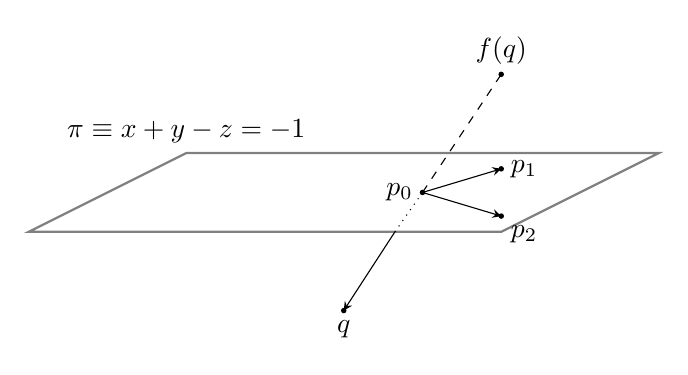
\begin{tikzpicture}
            % Definir los vértices del romboide
            \coordinate (A) at (0,0);
            \coordinate (B) at (2,1);
            \coordinate (C) at (8,1);
            \coordinate (D) at  (6,0);
        
            \coordinate (f_Q) at  (6,2);
            \coordinate (Q) at  (4,-1);
        
            \coordinate (p_0) at  (5,0.5);
            \coordinate (p_1) at  (6,0.8);
            \coordinate (p_2) at  (6,0.2);
        
            % Dibujar el romboide
            \draw[gray, thick] (A) -- (B) -- (C) -- (D) -- cycle;
            \node[above] at (B) {$\pi\equiv x+y-z=-1$};
            
            % Dibujar el punto arriba
            \fill (Q) circle (1pt);
            \node[below] at (Q) {$q$};
            
            % Dibujar el punto abajo
            \fill (f_Q) circle (1pt);
            \node[above] at (f_Q) {$f(q)$};
            
            % Dibujar el punto en el plano
            \fill (p_0) circle (1pt);
            \node[left] at (p_0) {$p_0$};
        
            % Dibujar el punto en el plano
            \fill (p_1) circle (1pt);
            \node[right] at (p_1) {$p_1$};
        
            % Dibujar el punto en el plano
            \fill (p_2) circle (1pt);
            \node[below right] at (p_2) {$p_2$};
        
            \draw[dashed] (p_0) -- (f_Q);
            \draw[dotted] (4.65,0) -- (p_0);
            
            \draw[-stealth] (4.65, 0) -- (Q);
            \draw[-stealth] (p_0) -- (p_1);
            \draw[-stealth] (p_0) -- (p_2);
        \end{tikzpicture}
    \end{figure}

    Consideramos dos vectores de $\vec{\pi}$ linealmente independientes:
    \begin{equation*}
        v_1 = (1,0,1) \qquad v_2 = (0,1,1)
    \end{equation*}

    Sea ahora $p_0=(-1,-1,-1)\in \pi$ y $q=(0,0,0)\in \bb{R}^2$. Sea entonces el tercer vector de la base $v_3=\vec{p_0q} = (1,1,1)$. Comprobemos que los tres vectores son linealmente independientes:
    \begin{equation*}
        \left|\begin{array}{ccc}
            1 & 0 & 1 \\
            0 & 1 & 1\\
            1 & 1 & 1
        \end{array}\right| = 1 - 1 -1 = -1\neq 0
    \end{equation*}
    Por tanto, forman base. Tomamos el sistema de referencia $\cc{R}=\{p_0, \cc{B}=\{v_1,v_2,v_3\}\}$. Tenemos que $f(p_0)=p_0$ por ser un punto fijo, por lo que $f(p_0)=(0,0,0)_{\cc{R}}$. Calculamos ahora las imágenes mediante $\vec{f}$ de los vectores de la base.

    Tenemos que $v_i=\vec{p_0p_i}$, con $p_i\in \pi$ para $i=1,2$. Entonces,
    \begin{equation*}
        \vec{f}(v_i) = \vec{f(p_0)f(p_i)} = \vec{p_0p_i} = v_i \qquad i=1,2
    \end{equation*}

    Además, tenemos que:
    \begin{equation*}
        \vec{f}(v_3) = \vec{f(p_0)f(q)} = \vec{p_0(1,1,1)} = (2,2,2) = 2v_3
    \end{equation*}

    Entonces, la matriz asociada a $f$ es:
    \begin{equation*}
        M(f,\cc{R}) = \left(
        \begin{array}{c|ccc}
            1 & 0 & 0 & 0 \\ \hline
            0 & 1 & 0 & 0 \\
            0 & 0 & 1 & 0 \\
            0 & 0 & 0 & 2
        \end{array} \right)
    \end{equation*}

    Como la matriz asociada a $\vec{f}$ es regular, tenemos que $\vec{f}$ es biyectiva; y por tanto $f$ también lo es.

    Para obtener la matriz asociada a $f$ en $\cc{R}_0$, usamos que:
    \begin{equation*}
        M(Id_{\bb{R}^3},\cc{R}, \cc{R}_0) = \left(
        \begin{array}{c|ccc}
            1 & 0 & 0 & 0 \\ \hline
            -1 & 1 & 0 & 1 \\
            -1 & 0 & 1 & 1 \\
            -1 & 1 & 1 & 1
        \end{array} \right)
    \end{equation*}

    Entonces, tenemos que:
    \begin{equation*}\begin{split}
        M(f,\cc{R}_0) &= M(Id_{\bb{R}^3}, \cc{R}, \cc{R}_0)\cdot M(f,\cc{R}) \cdot M(Id_{\bb{R}^3}, \cc{R}_0, \cc{R})=\\&
        = \left(
        \begin{array}{c|ccc}
            1 & 0 & 0 & 0 \\ \hline
            -1 & 1 & 0 & 1 \\
            -1 & 0 & 1 & 1 \\
            -1 & 1 & 1 & 1
        \end{array} \right)
        \left(
        \begin{array}{c|ccc}
            1 & 0 & 0 & 0 \\ \hline
            0 & 1 & 0 & 0 \\
            0 & 0 & 1 & 0 \\
            0 & 0 & 0 & 2
        \end{array} \right)
        \left(
        \begin{array}{c|ccc}
            1 & 0 & 0 & 0 \\ \hline
            -1 & 1 & 0 & 1 \\
            -1 & 0 & 1 & 1 \\
            -1 & 1 & 1 & 1
        \end{array} \right)^{-1} =\\&
        = \left(
        \begin{array}{c|ccc}
            1&	0	&0&	 0 \\ \hline
            1&	2&	1&	-1 \\
            1&	1&	2&	-1 \\
            1&	1&	1&	 0 \\
        \end{array} \right)
    \end{split}\end{equation*}
    
\end{ejercicio}

\begin{ejercicio}
    Consideremos los sistemas de referencia de $\bb{R}^2$ dados por
    \begin{equation*}
        \cc{R} = \{(1, 1), (2, 1), (2, 2)\}
        \qquad \text{y} \qquad
        \cc{R}' = \{(1, 0), (0, 0), (-1, -1)\}.
    \end{equation*}

    Sea $f:\bb{R}^2\to \bb{R}^2$ la única aplicación afín tal que
    \begin{equation*}
        f (1, 1) = (3, 3),\qquad f (2, 1) = (3, -1),\qquad f (2, 2) = (2, 0).
    \end{equation*}

    Calcula las ecuaciones que representan a $f$ respecto de los sistemas de referencia $\cc{R}$ (en el dominio) y $\cc{R}'$ (en el codominio), y las ecuaciones que representan a $f$ respecto de los sistemas de referencia usuales. ¿Cuál es la imagen del punto $(5, 5)$?\\

    Sea $\cc{R}=\{(1,1),\cc{B}=\{(1,0), (1,1)\}\}$, $\cc{R}'=\{(1,0), \cc{B}'=(-1,0), (-2, -1)\}$. De forma directa, podemos obtener $M(f,\cc{R},\cc{R}_0)$. Tenemos que:
    \begin{gather*}
        \vec{f}(1,0) = \vec{f(1,1)f(2,1)} = \vec{(3,3)(3,-1)} = (0,-4)\\
        \vec{f}(1,1) = \vec{f(1,1)f(2,2)} = \vec{(3,3)(2,0)} = (-1,-3)
    \end{gather*}

    Por tanto,
    \begin{equation*}
        M(f,\cc{R},\cc{R}_0) = 
        \left(\begin{array}{c|cc}
            1 & 0 & 0 \\ \hline
            3 & 0 & -1\\
            3 & -4 & -3
        \end{array}\right)
    \end{equation*}

    Para obtener las ecuaciones en los sistemas de referencia pedidos, calculamos las matrices de cambio de base necesarias:
    \begin{equation*}\begin{split}
        M(f,\cc{R},\cc{R}') &= M(Id_{\cc{R}^2}, \cc{R}_0, \cc{R}')\cdot M(f,\cc{R},\cc{R}_0) =\\
        &= M(Id_{\cc{R}^2}, \cc{R}', \cc{R}_0)^{-1}\cdot M(f,\cc{R},\cc{R}_0) =\\
        &= \left(\begin{array}{c|cc}
            1 & 0 & 0 \\ \hline
            1 & -1 & -2\\
            0 & 0 & -1
        \end{array}\right)^{-1}
        \left(\begin{array}{c|cc}
            1 & 0 & 0 \\ \hline
            3 & 0 & -1\\
            3 & -4 & -3
        \end{array}\right) =\\
        &= \left(\begin{array}{c|cc}
            1 & 0 & 0 \\ \hline
            4 & -8 & -5\\
            -3 & 4 & 3
        \end{array}\right)
    \end{split}\end{equation*}

    Para las ecuaciones en los sistemas de referencia usuales, tenemos que:
    \begin{equation*}\begin{split}
        M(f,\cc{R}_0,\cc{R}_0) &=M(f,\cc{R},\cc{R}_0)\cdot  M(Id_{\cc{R}^2}, \cc{R}_0, \cc{R}) =\\
        &= M(f,\cc{R},\cc{R}_0)\cdot  M(Id_{\cc{R}^2}, \cc{R}, \cc{R}_0)^{-1} =\\
        &= \left(\begin{array}{c|cc}
            1 & 0 & 0 \\ \hline
            3 & 0 & -1\\
            3 & -4 & -3
        \end{array}\right)\left(\begin{array}{c|cc}
            1 & 0 & 0 \\ \hline
            1 & 1 & 1\\
            1 & 0 & 1
        \end{array}\right)^{-1}
        =\\
        &= \left(\begin{array}{c|cc}
            1 & 0 & 0 \\ \hline
            4 & 0 & -1\\
            6 & -4 & 1
        \end{array}\right)
    \end{split}\end{equation*}
\end{ejercicio}


\begin{ejercicio}
    Sean $\cc{A}$ un espacio afín, $f : \cc{A} \to \cc{A}$ una aplicación afín y el subespacio $S = p_0 + \cc{L}\{v_0\}$ una recta en $\cc{A}$. Demuestra que $f(S) = S$ si y solo si $\vec{p_0~f(p_0)} \in \cc{L}\{v_0\}$ y $v_0$ es un vector propio de $\vec{f}$ de valor propio no nulo.
    \begin{description}
        \item[$\Longrightarrow)$] Suponemos que $f$ deja invariante a la recta. Entonces, como $p_0\in S$, entonces $f(p_0)\in S$, por lo que $\vec{p_0~f(p_0)}\in \vec{S}=\cc{L}\{v_0\}$. Veamos ahora que $v_0$ es un vector propio de $\vec{f}$ de valor propio no nulo.

        Para ver esto, veamos en primer lugar que $\exists p\in S$ tal que $f(p)\neq f(p_0)$. Si fuese $f(p)=f(p_0)$ para todo $p\in S$, tendríamos que $f(S)=f(p_0)$ un único punto, que no es posible ya que $f(S)$ es una recta. Por tanto, $\exists p\in S$ tal que $f(p)\neq f(p_0)$.

        Como $f(p)\neq f(p_0)$, entonces $p\neq p_0$. Entonces, $\vec{pp_0}\in S$ no es nulo, por lo que $\vec{pp_0}=\lambda_1 v_0$, con $\lambda\in \bb{R}^\ast$. Entonces, tenemos que:
        \begin{equation*}
            \begin{split}
                \vec{f}(\vec{pp_0}) &\stackrel{(1)}{=} \vec{f}(\lambda_1 v_0) = \lambda_1 \vec{f}(v_0) \\
                    &\stackrel{(2)}{=} \vec{f(p)f(p_0)} = \lambda_2 v_0
            \end{split}
        \end{equation*}
        Donde en $(1)$ he aplicado lo visto anteriormente, y en $(2)$ he aplicado la definición de aplicación lineal asociada y que, como $p,p_0\in S$, sus imágenes pertenecen a $S$ y, por tanto, dicho vector a $\vec{S}$. Además, como $f(p)\neq f(p_0)$, no es nulo, por lo que $\lambda_2\in \bb{R}^\ast$.

        Entonces, tenemos que:
        \begin{equation*}
            \vec{f}(v_0) = \frac{\lambda_2}{\lambda_1} v_0
        \end{equation*}
        con $\lambda = \dfrac{\lambda_2}{\lambda_1}\in \bb{R}^\ast$ valor propio, que no es nulo ya que $\lambda_1,\lambda_2\neq 0$.

        \item[$\Longleftarrow)$] Veamos en primer lugar que $f(p_0)\in S$. Tenemos que $\vec{p_0~f(p_0)}=\lambda v_0$, con $\lambda\in \bb{R}$. Entonces, $f(p_0)=p_0+\lambda v_0\in S$, por lo que se tiene.

        Además, por hipótesis $v_0$ es un vector propio de $\vec{f}$ con valor propio $\lambda_1\in \bb{R}^\ast$, por lo que $\vec{f}(v_0) = \lambda_1 v_0$.

        Demostramos la doble inclusión:
        \begin{description}
            \item[$\subset)$] Sea $p\in S$. Si $p=p_0$, tenemos que $f(p)\in S$, por lo que descartamos este caso inicial. Si $p\neq p_0$, entonces $p=p_0+\lambda_2 v_0$, con $\lambda_2 \in \bb{R}^\ast$. Entonces,
            \begin{equation*}
                f(p)=f(p_0) + \lambda_2\vec{f}(v_0) = f(p_0) +\lambda_2 \lambda_1 v_0\in S
            \end{equation*}

            Por tanto, tengo que $f(S)\subset S$.
            
            \item[$\supset)$] Sea $q\in S$. Veamos que $\exists p\in S$ tal que $f(p)=q$. Tenemos que:
            \begin{equation*}
                \begin{split}
                    q &= p_0+\lambda_2 v_0+f(p_0)-f(p_0) = -\vec{p_0f(p_0)} + \lambda_2 v_0 + f(p_0) =\\
                    &= \lambda_3 v_0 + f(p_0)
                    = \lambda_3\cdot \frac{\lm_1}{\lm_1}\cdot   v_0 + f(p_0) 
                    =\frac{\lm_3}{\lm_1}\cdot \vec{f}(v_0) + f(p_0) 
                    =\\&= f\left(p_0 + \frac{\lm_3}{\lm_1}\cdot v_0\right)
                \end{split}
            \end{equation*}

            Definiendo $p=p_0+\frac{\lm_3}{\lm}\cdot v_0\in S$, tenemos que $f(p)=q$. Por tanto, $q\in f(S)$.
        \end{description}

        Entonces, $f(S)=S$.        
    \end{description}
\end{ejercicio}


\begin{ejercicio}
    Sean $\cc{A}$ un plano afín, $f : \cc{A} \to \cc{A}$ una aplicación afín y ${R}_1, {R}_2, {R}_3$ tres rectas distintas donde no hay dos paralelas. Prueba que si $f(R_i) \| R_i,~i = 1, 2, 3$, entonces $f$ es una traslación o una homotecia.\\

    Sean las rectas $R_i=p_i+\cc{L}\{v_i\}$ para $i=1,2,3$. Para todo $i=1,2,3$ y para todo $v_i\in \vec{R_i}$,
    se tiene que:
    \begin{equation*}
        \vec{f}(v_i) \in {\vec{f}\left(\vec{R_i}\right)} = \vec{R_i} \Longrightarrow \vec{f}(v_i) = \lambda_i v_i
        \qquad\text{ con } \lambda_i\in \bb{R}^\ast
    \end{equation*}

    Distinguimos en función de si las tres rectas son concurrentes o no:
    \begin{itemize}
        \item \ul{Supongamos que no son concurrentes}:
        
        Sea $R_1\cap R_2 = \{p_{12}\}$, que sabemos que se cortan por no ser paralelas. Análogamente, sean $R_1\cap R_3 = \{p_{13}\}$, $R_2\cap R_3 = \{p_{23}\}$.
        Como no son concurrentes, dichos puntos son distintos dos a dos. Consideramos ahora los vectores $\vec{p_{12}p_{13}}\in \vec{R_1}$, $\vec{p_{12}p_{23}}\in \vec{R_2}$,
        $\vec{p_{13}p_{23}}\in \vec{R_3}$. Entonces, tenemos que:
        \begin{equation*}
            \vec{f}(\vec{p_{12}p_{13}}) = \lambda_1~ \vec{p_{12}p_{13}} \qquad
            \vec{f}(\vec{p_{12}p_{23}}) = \lambda_2~ \vec{p_{12}p_{23}} \qquad
            \vec{f}(\vec{p_{13}p_{23}}) = \lambda_3~ \vec{p_{13}p_{23}}
        \end{equation*}

        Además, por la igualdad triangular, tenemos que $\vec{p_{12}p_{13}}+\vec{p_{13}p_{23}}=\vec{p_{12}p_{23}}$, por lo que:
        \begin{equation*}
            \begin{split}
                \vec{f}(\vec{p_{12}p_{23}}) &= \vec{f}(\vec{p_{12}p_{13}}+\vec{p_{13}p_{23}}) = \vec{f}(\vec{p_{12}p_{13}})+\vec{f}(\vec{p_{13}p_{23}}) =\\
                &= \lambda_1~ \vec{p_{12}p_{13}} + \lambda_3~ \vec{p_{13}p_{23}}
            \end{split}
        \end{equation*}

        Por tanto, tenemos que:
        \begin{multline*}
            \lambda_1~ \vec{p_{12}p_{13}} + \lambda_3~ \vec{p_{13}p_{23}} =
            \lambda_2~ \vec{p_{12}p_{23}} = \lm_2~\vec{p_{12}p_{13}} + \lm_2~\vec{p_{13}p_{23}}
            \Longrightarrow \\ \Longrightarrow (\lambda_1-\lambda_2)~ \vec{p_{12}p_{13}} + (\lambda_3-\lambda_2)~ \vec{p_{13}p_{23}} = 0
        \end{multline*}

        Como $R_1\not\|R_3$, tenemos que $\{\vec{p_{12}p_{13}}, \vec{p_{13}p_{23}}\}$ son linealmente independientes por ser ambos no nulos, por lo que:
        $\lambda_1-\lambda_2 = \lambda_3-\lambda_2 = 0$, y entonces $\lambda_1=\lambda_2=\lambda_3=\lambda \in \bb{R}^\ast$.

        Como $\{\vec{p_{12}p_{13}}, \vec{p_{13}p_{23}}\}$ forman base de $\cc{A}$ y $\vec{f}$ es lineal, tenemos que:
        \begin{equation*}
            \vec{f}(v) = \vec{f}\left(\alpha_1 \vec{p_{12}p_{13}} + \alpha_2 \vec{p_{13}p_{23}}\right)
            = \alpha_1 \lambda \vec{p_{12}p_{13}} + \alpha_2 \lambda \vec{p_{13}p_{23}} = \lambda v
        \end{equation*}

        Es decir, $\vec{f}=\lm Id$, por lo que $f$ es una homotecia o una traslación.

        \item \ul{Supongamos que son concurrentes}:
        
        Sea entonces $p\in R_1\cap R_2\cap R_3$, y consideramos $p_i\in R_i$, de forma que $\vec{pp_i}\in \vec{R_i}$ para $i=1,2,3$.
        Entonces, tenemos que:
        \begin{equation*}
            \vec{f}(\vec{pp_1}) = \lambda_1~ \vec{pp_1} \qquad
            \vec{f}(\vec{pp_2}) = \lambda_2~ \vec{pp_2} \qquad
            \vec{f}(\vec{pp_3}) = \lambda_3~ \vec{pp_3}
        \end{equation*}

        Además, consideramos la base de $\cc{A}$ $\{\vec{pp_1}, \vec{pp_2}\}$. Entonces, tenemos que:
        \begin{equation*}
            \vec{pp_3} = \alpha \vec{pp_1} + \beta \vec{pp_2}, \qquad \alpha,\beta\in \bb{R}^\ast
        \end{equation*}
        donde sabemos que $\alpha, \beta\neq 0$ ya que si alguno de ellos fuese nulo,
        entonces pertenecería a $R_1$ o a $R_2$, y entonces $R_1\|R_3$ o $R_2\|R_3$, lo cual no es una contradicción.
        Por tanto, tenemos que:
        \begin{align*}
            \vec{f}\left(\vec{pp_3}\right) &
            = \vec{f}\left(\alpha \vec{pp_1} + \beta \vec{pp_2}\right)
            = \alpha \vec{f}\left(\vec{pp_1}\right) + \beta \vec{f}\left(\vec{pp_2}\right)
            = \alpha \lambda_1 \vec{pp_1} + \beta \lambda_2 \vec{pp_2}\\&
            = \lm_3 \left(\alpha \vec{pp_1} + \beta \vec{pp_2}\right)
            = \lm_3 \alpha \vec{pp_1} + \lm_3 \beta \vec{pp_2}
        \end{align*}

        Por tanto, pasando todo al mismo miembro, tenemos que:
        \begin{equation*}
            \alpha\left(\lambda_1-\lambda_3\alpha\right) \vec{pp_1} + \beta\left(\lambda_2-\lambda_3\beta\right) \vec{pp_2} = 0
        \end{equation*}

        Como $\{\vec{pp_1}, \vec{pp_2}\}$ son linealmente independientes, tenemos que:
        \begin{equation*}
            \alpha\left(\lambda_1-\lambda_3\alpha\right) = \beta\left(\lambda_2-\lambda_3\beta\right) = 0
        \end{equation*}

        Además, como $\alpha,\beta\neq 0$, tenemos que $\lambda_1=\lambda_3=\lambda_2=\lambda\in \bb{R}^\ast$.
        Por tanto, tenemos que:
        \begin{equation*}
            \vec{f}(v) = \vec{f}\left(\alpha \vec{pp_1} + \beta \vec{pp_2}\right)
            = \alpha \lambda \vec{pp_1} + \beta \lambda \vec{pp_2} = \lambda v
        \end{equation*}

        Es decir, $\vec{f}=\lm Id$, por lo que $f$ es una homotecia o una traslación.
    \end{itemize}
\end{ejercicio}

\begin{ejercicio}
    Sea $\cc{A}$ un espacio afín, $f:\cc{A}\to \cc{A}$ una aplicación afín y biyectiva que lleva rectas de $\cc{A}$ en rectas paralelas, es decir:
    \begin{equation*}
        r\|f(r) \qquad \forall r\subset \cc{A},~ \dim r =1
    \end{equation*}
    Demostrar que $f$ es una dilatación.\\

    Por el ejercicio anterior, tan solo es necesario ver que es posible tomar tres rectas
    $R_1,R_2,R_3$ distintas tales que no haya dos paralelas.
    Para ello, tomamos $R_1$ cualquiera, y $R_2$ y $R_3$ tales que $R_2\cap R_1 = \{p_1\}$ y
    $R_3\cap R_1 = \{p_2\}$, con $p_1\neq p_2$. Entonces, $R_2\cap R_3 = \{p_3\}$, con $p_3\neq p_1,p_2$.
\end{ejercicio}

\begin{ejercicio}
    Sea $f : \cc{A} \to \cc{A}$ una aplicación afín de un espacio afín  $\cc{A}$ en sí mismo. Consideremos el subespacio vectorial $\cc{W} = \left\{v \in \vec{\cc{A}} \mid \vec{f}(v) = v\right\}$. Demuestra que
    \begin{enumerate}
        \item El conjunto de puntos fijos de $f$ es vacío o un subespacio afín cuyo espacio de direcciones es $\cc{W}$.
        
        Supongamos $\cc{P}_f\neq \emptyset$, y sea $q \in \cc{P}_f$. Entonces, dado $p\in \cc{A}$, tenemos que:
        \begin{equation*}
            p\in \cc{P}_f \Longleftrightarrow f(p)=p \Longleftrightarrow \vec{pq} = \vec{f(p)q} = \vec{f(p)f(q)} = \vec{f}\left(\vec{pq}\right) \Longleftrightarrow \vec{pq}\in \cc{W}
        \end{equation*}
        
        Por tanto, $\cc{P}_f = q + \cc{W}$, por lo que es un subespacio afín de espacio de direcciones $\cc{W}$.
        
        \item Si $\cc{W} = \left\{\vec{0}\right\}$ entonces $f$ tiene un único punto fijo.
        
        Supongamos demostrado la existencia, y veamos la unicidad. Supongamos que $f$ tiene dos puntos fijos $p_1,p_2$.
        Entonces, tenemos que $\vec{p_1p_2}\in \vec{\cc{P}_f}=\cc{W}=\left\{\vec{0}\right\}$, por lo que $p_1=p_2$, quedando demostrada la unicidad.

        Veamos ahora la existencia del punto fijo. Fijado $p\in \cc{A}$, supongamos que existe $q\in \cc{A}$ tal que $f(q)=q$. Entonces, tenemos que:
        \begin{align*}
            f(q)=q &\Longleftrightarrow \vec{qf(q)}=\vec{0}
            \Longleftrightarrow \vec{qp}+\vec{pf(p)} + \vec{f(p)f(q)} = \vec{0} \Longleftrightarrow \\
            &\Longleftrightarrow Id_{\vec{\cc{A}}}\left(\vec{qp}\right)+\vec{pf(p)} + \vec{f}\left(\vec{pq}\right) = \vec{0}\Longleftrightarrow \\
            &\Longleftrightarrow \vec{f}\left(\vec{pq}\right) - Id_{\vec{\cc{A}}}\left(\vec{pq}\right) = \vec{f(p)p}\Longleftrightarrow \\
            &\Longleftrightarrow \left(\vec{f} - Id_{\vec{\cc{A}}}\right) \left(\vec{pq}\right) = \vec{f(p)p}\Longleftrightarrow \\
            &\Longleftrightarrow \vec{pq} = \left(\vec{f} - Id_{\vec{\cc{A}}}\right)^{-1}\left(\vec{f(p)p}\right)\Longleftrightarrow \\
            &\Longleftrightarrow q = p + \left(\vec{f} - Id_{\vec{\cc{A}}}\right)^{-1}\left(\vec{f(p)p}\right)
        \end{align*}

        Por tanto, mediante este razonamiento heurístico\footnote{Este razonamiento se denomina heurístico porque hemos 
        comenzado suponiendo lo que buscábamos demostrar. Otras veces, este tipo de razonamientos se encuentran dando directamente el punto,
        y viendo que cumple que es un punto fijo. Es análogo, pero se ha optado por esta forma, para que así el lector vea
        que ese valor de $q$ no es suerte ni ``magia''.}, hemos obtenido que, fijado $p\in \cc{A}$, el siguiente punto es un punto fijo de $f$:
        \begin{equation*}
            q:= p + \left(\vec{f} - Id_{\vec{\cc{A}}}\right)^{-1}\left(\vec{f(p)p}\right)
        \end{equation*}

        Por tanto, queda también demostrada la existencia.       
    \end{enumerate}
\end{ejercicio}

\begin{ejercicio}
    Consideremos $k + 1$ puntos $p_0, p_1, \dots , p_k$ de un espacio afín $\cc{A}$. Definimos el baricentro de estos puntos como
    \begin{equation*}
        b=p_0+\frac{1}{k+1} \sum_{i=0}^k \vec{p_0p_i}.
    \end{equation*}

    Demuestra que $b$ no depende del punto inicial $p_0$ elegido. (Cuando $k = 1$ el punto $b$ se le denomina el punto medio de $p_0$ y $p_1$).\\

    Sea $p_0'\in \{p_0,\dots,p_k\}$ otro punto. Entonces, tenemos que:
    \begin{equation*}\begin{split}
        p_0+&\frac{1}{k+1}\sum_{i=0}^k \vec{p_0p_i} = p_0'+ \frac{1}{k+1}\sum_{i=0}^k \vec{p_0'p_i} \Longleftrightarrow \\
        &\Longleftrightarrow p_0-p_0' = \frac{1}{k+1}\sum_{i=0}^{k}\left(\vec{p_0'p_i} - \vec{p_0p_i}\right) \Longleftrightarrow\\
        &\Longleftrightarrow p_0-p_0' = \frac{1}{k+0}\sum_{i=0}^{k}\vec{p_0'p_0} \Longleftrightarrow\\
        &\Longleftrightarrow \vec{p_0'p_0} = \frac{k+1}{k+1}\vec{p_0'p_0} \Longleftrightarrow\\
        &\Longleftrightarrow \vec{p_0'p_0} = \vec{p_0'p_0}
    \end{split}\end{equation*}

    Por tanto, hemos obtenido que $b$ no depende del punto inicial elegido. Como observación, siempre podemos reordenar los puntos para que $p_0'$ sea el primer punto, de forma que la sumatoria empiece en $i=1$.
\end{ejercicio}

\begin{ejercicio}
    Sea $f : \cc{A} \to \cc{A}'$ una aplicación afín entre dos espacios afines. Si $b \in A$ es el baricentro de los puntos $p_0, p_1, \dots , p_k \in \cc{A}$, demuestra que $f (b)$ es el baricentro de los puntos $f (p_0), f (p_1), \dots , f (p_k)$.

    \begin{equation*}
        \begin{split}
            f(b) &= f\left(p_0+\frac{1}{k+1}\sum_{i=0}^k \vec{p_0p_i}\right) = f(p_0)+\vec{f}\left(\frac{1}{k+1}\sum_{i=0}^k \vec{p_0p_i}\right) =\\
            &= f(p_0)+\frac{1}{k+1}\sum_{i=0}^k \vec{f}(\vec{p_0p_i}) = f(p_0)+\frac{1}{k+1}\sum_{i=0}^k \vec{f(p_0)f(p_i)}
        \end{split}
    \end{equation*}
    Por tanto, hemos obtenido que $f(b)$ es el baricentro de los puntos $f(p_0), f(p_1), \dots , f(p_k)$.
\end{ejercicio}

\begin{ejercicio}
    Un triángulo en un espacio afín son tres puntos afínmente independientes. Prueba que las tres medianas de un triángulo se cortan en el baricentro de sus vértices, donde se llama mediana a cada recta que pasa por un vértice y el punto medio de los otros dos.\\

    Demostrado en el Teorema \ref{teo:baricentro}.
\end{ejercicio}

\begin{ejercicio}
    Sea $T_1$ un triángulo en un plano afín $\cc{A}$ y $T_2$ el triángulo cuyos vértices son los tres puntos medios de los vértices de $T_1$. Prueba que $T_1$ y $T_2$ tienen lados paralelos e igual baricentro. Calcula el centro y razón de la homotecia en $\cc{A}$ que transforma $T_2$ en $T_1$.

    En el Teorema \ref{teo:euler}, se demostró que el centro de homotecia es el baricentro, y la razón es $-\frac{1}{2}$.
    Como una homotecia lleva rectas en rectas paralelas, tenemos que los lados de $T_1$ y $T_2$ son paralelos.
\end{ejercicio}

\begin{ejercicio}\label{ej:5.1.36}
    Sean $\cc{A}$ un espacio afín y $a_0, a_1, a_2 \in A$ los vértices de un triángulo con baricentro $b \in \cc{A}$. Sean $a_3, a_4 \in \cc{A}$ los puntos intersección del lado que contiene a $a_1$ y $a_2$ con las rectas paralelas a los otros dos lados pasando por $b$. Demuestra que, salvo reordenación de los puntos $a_3, a_4$, se tiene que
    \begin{equation*}
        \vec{a_1a_3} = \vec{a_3a_4}= \vec{a_4a_2} = \frac{1}{3} \cdot \vec{a_1a_2}
    \end{equation*}

    \begin{figure}[H]
        \centering
        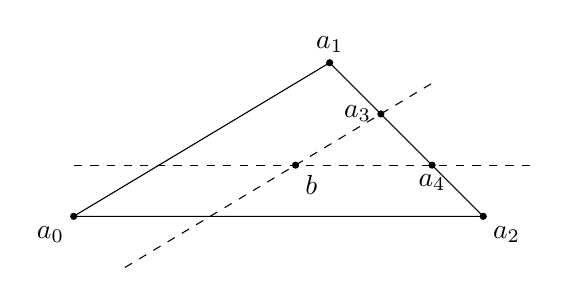
\begin{tikzpicture}[scale=1.3]
            % Puntos del triángulo
            \coordinate (a0) at (0,0);
            \coordinate (a1) at (2.5,1.5);
            \coordinate (a2) at (4,0);

            % Punto B
            \coordinate (b) at (13/6,0.5);

            % Puntos a3, a4
            \coordinate (a3) at (3,1);
            \coordinate (a4) at (3.5,0.5);

            % Puntos de inicio y final de las rectas
            \coordinate (Ra0a2'_init) at (0, 0.5);
            \coordinate (Ra0a2'_end) at (4.5, 0.5);
            \coordinate (Ra0a1'_init) at (0.5,-0.5);
            \coordinate (Ra0a1'_end) at (3.5, 1.3);

            % Triángulo
            \draw (a0) -- (a1) -- (a2) -- cycle;

            % Rectas paralelas
            \draw[dashed] (Ra0a2'_init) -- (Ra0a2'_end);
            \draw[dashed] (Ra0a1'_init) -- (Ra0a1'_end);

            % Puntos
            \fill (a0) circle (1pt) node[anchor=north east] {$a_0$};
            \fill (a1) circle (1pt) node[anchor=south] {$a_1$};
            \fill (a2) circle (1pt) node[anchor=north west] {$a_2$};
            \fill (b) circle (1pt) node[anchor=north west] {$b$};
            \fill (a3) circle (1pt) node[left] {$a_3$};
            \fill (a4) circle (1pt) node[below] {$a_4$};
        \end{tikzpicture}  
        \caption{Ejercicio del ejercicio \ref{ej:5.1.36}.}      
    \end{figure}


    Por la definición de baricentro, como $b$ es el baricentro de $a_0,a_1,a_2$, y no depende del punto inicial elegido, tenemos que:
    \begin{equation*}
        b = a_1 + \frac{1}{3}\left(\vec{a_1a_0} + \vec{a_1a_2}\right)
        = a_2 + \frac{1}{3}\left(\vec{a_2a_0} + \vec{a_2a_1}\right)
    \end{equation*}

    Como $a_3\in a_1+\cc{L}\{\vec{a_1a_2}\}$, entonces $\vec{a_1a_3} = \mu \vec{a_1a_2}$, con $\mu \in \bb{R}$.
    Además, como $a_3\in b+\cc{L}\{\vec{a_0a_1}\}$, entonces $a_3 = b + \lambda \vec{a_0a_1}$, con $\lambda \in \bb{R}$. De la definición de $b$, tenemos que
    $a_3 = a_1 + \frac{1}{3}\left(\vec{a_1a_0} + \vec{a_1a_2}\right) + \lambda \vec{a_0a_1}$,
    por lo que $\vec{a_1a_3} = \frac{1}{3}\left(\vec{a_1a_0} + \vec{a_1a_2}\right) + \lambda \vec{a_0a_1}$. Igualando con lo obtenido anteriormente, tenemos que:
    \begin{multline*}
        \mu \vec{a_1a_2} = \frac{1}{3}\left(\vec{a_1a_0} + \vec{a_1a_2}\right) + \lambda \vec{a_0a_1} \Longrightarrow \\
        \Longrightarrow \frac{1}{3}\left(\vec{a_1a_0} + \vec{a_1a_2}\right) -\lm \vec{a_1a_0} - \mu \vec{a_1a_2} = 0 \Longrightarrow\\
        \Longrightarrow \left(\frac{1}{3}-\lm\right) \vec{a_1a_0} + \left(\frac{1}{3}-\mu\right) \vec{a_1a_2} = 0 
    \end{multline*}

    Como $a_0,a_1,a_2$ son afínmente independientes, tenemos que $\vec{a_1a_0}, \vec{a_1a_2}$ son linealmente independientes, por lo que:
    \begin{equation*}
        \left(\frac{1}{3}-\lm\right) = \left(\frac{1}{3}-\mu\right) = 0 \Longrightarrow \lm = \mu = \frac{1}{3}
    \end{equation*}

    Por tanto, $\vec{a_1a_3} = \frac{1}{3}\vec{a_1a_2}$. Trabajemos ahora con $a_4$.\\

    Como $a_4\in a_2+\cc{L}\{\vec{a_1a_2}\}$, entonces $\vec{a_4a_2} = \mu' \vec{a_1a_2}$, con $\mu' \in \bb{R}$.
    Además, como $a_4\in b+\cc{L}\{\vec{a_0a_2}\}$, entonces $a_4 = b + \lambda' \vec{a_0a_2}$, con $\lambda' \in \bb{R}$. De la definición de $b$, tenemos que
    $a_4 = a_2 + \frac{1}{3}\left(\vec{a_2a_0} + \vec{a_2a_1}\right) + \lambda' \vec{a_0a_2}$,
    por lo que $\vec{a_2a_4} = \frac{1}{3}\left(\vec{a_2a_0} + \vec{a_2a_1}\right) + \lambda' \vec{a_0a_2}$. Igualando con lo obtenido anteriormente, tenemos que:
    \begin{multline*}
        \mu' \vec{a_1a_2} = -\frac{1}{3}\left(\vec{a_2a_0} + \vec{a_2a_1}\right) - \lambda' \vec{a_0a_2} \Longrightarrow \\
        \Longrightarrow -\frac{1}{3}\left(\vec{a_2a_0} + \vec{a_2a_1}\right) +\lm' \vec{a_2a_0} + \mu' \vec{a_2a_1} = 0 \Longrightarrow\\
        \Longrightarrow \left(\lm' -\frac{1}{3}\right) \vec{a_2a_0} + \left(\mu'-\frac{1}{3}\right) \vec{a_2a_1} = 0 
    \end{multline*}

    Como $a_0,a_1,a_2$ son afínmente independientes, tenemos que $\vec{a_2a_0}, \vec{a_2a_1}$ son linealmente independientes, por lo que:
    \begin{equation*}
        \left(\lm' -\frac{1}{3}\right) = \left(\mu'-\frac{1}{3}\right) = 0 \Longrightarrow \lm' = \mu' = \frac{1}{3}
    \end{equation*}
    De esta forma, vemos también que $\vec{a_4a_2} = \frac{1}{3}\vec{a_1a_2}$. Por tanto:
    \begin{equation*}
        \vec{a_1a_2} \AstIg \vec{a_1a_3} + \vec{a_3a_4} + \vec{a_4a_2}
        = \frac{1}{3}\vec{a_1a_2} + \vec{a_3a_4} + \frac{1}{3}\vec{a_1a_2} \Longrightarrow \vec{a_4a_2} = \frac{1}{3}\vec{a_1a_2}
    \end{equation*}
    donde en $(\ast)$ he aplicado la igualdad triangular.

    Por tanto, hemos obtenido que $\vec{a_1a_3} = \vec{a_3a_4}= \vec{a_4a_2} = \frac{1}{3} \cdot \vec{a_1a_2}$, como queríamos demostrar.
\end{ejercicio}

\begin{ejercicio}
    Sean $\cc{A}$ un espacio afín de dimensión mayor o igual a dos y $f : \cc{A} \to \cc{A}$ una aplicación biyectiva (no necesariamente afín) que lleva rectas en rectas paralelas. Demuestra que
    \begin{enumerate}
        \item Toda recta que pasa por un punto fijo es una recta fija.

        Sea $r=p+\vec{r}$ una recta, es decir, $\dim \vec{r}=1$ y $p\in \cc{A}$. Entonces, como $f$ lleva rectas en rectas paralelas, tenemos que $$f(r)=f(p)+\vec{r} \qquad \forall p\in r$$

        Sea ahora $p_0$ el punto fijo, es decir, $f(p_0)=p_0$. Entonces:
        $$f(r)=f(p_0)+\vec{r}=p_0+\vec{r}=r$$

        Por tanto, como $f(r)=r$, tenemos que $f$ es una recta fija.

        
        \item La recta que pasa por un punto y su imagen es una recta fija.

        Sea ahora $r=p+\vec{r}$ una recta con $p_0,f(p_0)\in r$. Entonces, como ambos puntos están en la recta, tenemos que:
        $$r=p_0+\vec{r} \qquad r=f(p_0)+\vec{r}$$

        Calculemos ahora $f(r)$ para ver si es fija. Como $p_0\in r$ y $\vec{f(r)}=\vec{r}$:
        \begin{equation*}
            f(r)=f(p_0)+\vec{r}=r
        \end{equation*}

        Por tanto, como $f(r)=r$, tenemos que $f$ es una recta fija.
        
        \item Si $f$ tiene dos puntos fijos ha de ser la identidad.

        Sean $p_0,p_1\in \cc{A}$, $p_0\neq p_1$, los puntos fijos; es decir, $f(p_0)=p_0$ y $f(p_1)=p_1$. Consideramos ahora $q\in \cc{A}$. Realizamos distinción entre si los tres puntos están o no alineados:
        \begin{enumerate}
            \item Supongamos que no están alineados:

            Sean entonces $\vec{p_1q}, \vec{p_2q}\in \vec{\cc{A}}$ dos vectores linealmente independientes (lo son ya que no están alineados). Consideramos las rectas $L_1 = q+\cc{L}\{\vec{p_1q}\}$, $L_2 = q+\cc{L}\{\vec{p_2q}\}$.

            Como $p_1\in L_1$ y $p_1$ es un punto fijo, tenemos que $f(L_1)=L_1$. Análogamente, $f(L_2)=L_2$.

            Además, tenemos que $q\in L_1,L_2$, por lo que $\{q\}= L_1\cap L_2$. Como se tiene que $q\in L_1,$ entonces $f(q)\in L_1$, y análogamente $f(q)\in L_2$. Por tanto, $f(q)\in L_1\cap L_2 = \{q\}$, por lo que $f(q)=q$.
            
            Es decir, $f(q)=q$ para todo $q\in \cc{A}\setminus (p_0+\cc{L}\{\vec{p_0p_1}\})$, es decir, que no esté alineado con los puntos fijos $p_0,p_1$.

            \item Supongamos que están alineados:
            
            Consideramos $q'\in \cc{A}$ no alineado con $p_0,p_1,q$. Entonces, por lo visto anteriormente, $f(q')=q'$. Aplicamos ahora el razonamiento anterior a $q$ usando los puntos fijos $p_0,q'$, de forma que llegamos a que $f(q)=q$.
        \end{enumerate}

        Por tanto, $f(q)=q$ para todo $q\in \cc{A}$, es decir, $f$ es la identidad.
        
        \item Si $f$ tiene un único punto fijo ha de ser una homotecia.
        
        Sea $q\in \cc{A}$, $q\neq p_0$. Tenemos que la recta $r=q+\cc{L}\{\vec{p_0q}\}$ pasa por $p_0$ (punto fijo), por lo que es una recta fija.

        Buscamos saber el valor de $\vec{f}$ en un vector cualquiera. Como fijado $p_0$ tenemos que $\vec{\cc{A}}$ es biyectivo a $\cc{A}$, lo comprobamos con $\vec{p_0q}$, que es un vector cualquiera. Entonces, tenemos que:
        \begin{equation*}
            \vec{f}(\vec{p_0q}) = \vec{f(p_0)f(q)} = \vec{p_0f(q)} \in \vec{r} \Longrightarrow \vec{f}(\vec{p_0q}) = \lambda \vec{p_0q} \qquad \forall q\in \cc{A}
        \end{equation*}

        Es decir, tenemos que $\vec{f}(v)=\lm v$ para todo $v\in \vec{\cc{A}}$. Como $f$ es biyectiva, tenemos que $f(q)\neq f(p_0)$, por lo que $\lm\neq 0$. Además, como $f$ tiene un único punto fijo, $f(q)\neq q$, por lo que $\lm\neq 1$. Es decir, $\lm \in \bb{R}\setminus \{0,1\}$, por lo que $f$ es una homotecia.


        \item Si $f$ no tiene ningún punto fijo ha de ser una traslación.
        
        Sean $p,q\in \cc{A}$, $p\neq q$, y consideramos la recta $r=p+\cc{L}\{\vec{pq}\}$.

        Tenemos que:
        \begin{equation*}
            \vec{f}(\vec{pq}) = \vec{f(p)f(q)} \in \vec{f(r)} = \vec{r} \Longrightarrow \vec{f}(\vec{pq}) = \lambda \vec{pq} \qquad \forall p,q\in \cc{A}
        \end{equation*}

        Es decir, tenemos que $f(v)=\lm v$ para todo $v\in \vec{\cc{A}}$. Veamos que $\lm =1$:
        \begin{enumerate}
            \item Si $\lm=0$, entonces $f(q)=f(p)$ para todo $p,q\in \cc{A}$, por lo que $f$ no es biyectiva, contradicción.
            \item Si $\lm \in \bb{R}\setminus \{0,1\}$, entonces $f$ es una homotecia, por lo que tiene un punto fijo (el centro), contradicción.
        \end{enumerate}
        Por tanto, $\lm=1$, es decir, $\vec{f}=Id$. Como $f$ no tiene ningún punto fijo, entonces $f$ es una traslación.
    \end{enumerate}
\end{ejercicio}

\begin{ejercicio}\label{ej:5.1.38}
    Sean $T_1, T_2$ dos triángulos de un espacio afín $\cc{A}$, con vértices respectivos $a_1, b_1, c_1$ y $a_2, b_2, c_2$. Supongamos que los triángulos no tienen vértices comunes y las tres rectas $R_{a_1a_2}$, $R_{b_1b_2}$ y $R_{c_1c_2}$ son paralelas o se cortan en el mismo punto. Demuestra que si
    \begin{equation*}
        R_{a_1b_1} \| R_{a_2b_2}
        \quad \text{y} \quad
        R_{a_1c_1} \| R_{a_2c_2}
    \end{equation*}
    entonces $R_{b_1c_1} \| R_{b_2c_2}$.\\

    Estamos ante un resultado similar al Teorema de Desargues, por lo que tenemos la siguiente figura:
    \begin{figure}[H]
        \centering
        \begin{subfigure}{0.5\linewidth}
            \centering\hspace{-0.3cm}
            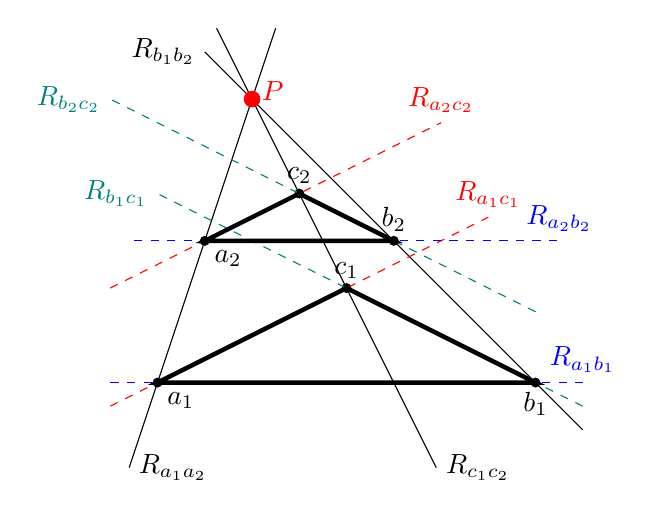
\begin{tikzpicture}[scale=0.6]
                % Los puntos del triángulo 1
                \coordinate (a_1) at (-4,0);
                \coordinate (b_1) at (4,0);
                \coordinate (c_1) at (0,2);

                % Los puntos del triángulo 2
                \coordinate (a_2) at (-3,3);
                \coordinate (b_2) at (1,3);
                \coordinate (c_2) at (-1,4);

                % Las rectas que unen los triángulos
                \coordinate (R_a1a2_ini) at (-4.6,-1.8);
                \coordinate (R_a1a2_fin) at (-1.5,7.5);

                \coordinate (R_c1c2_ini) at (1.9,-1.8);
                \coordinate (R_c1c2_fin) at (-2.75,7.5);

                \coordinate (R_b1b2_ini) at (5,-1);
                \coordinate (R_b1b2_fin) at (-3,7);

                % Las rectas que unen los vértices del triángulo 1
                \coordinate (R_a1b1_ini) at (-5,-0.5);
                \coordinate (R_a1b1_fin) at (3,3.5);

                \coordinate (R_a1c1_ini) at (-5,0);
                \coordinate (R_a1c1_fin) at (5,0);

                \coordinate (R_b1c1_ini) at (5,-0.5);
                \coordinate (R_b1c1_fin) at (-4,4);

                % Las rectas que unen los vértices del triángulo 2
                \coordinate (R_a2b2_ini) at (-5,2);
                \coordinate (R_a2b2_fin) at (2,5.5);

                \coordinate (R_a2c2_ini) at (-4.5,3);
                \coordinate (R_a2c2_fin) at (4.5,3);

                \coordinate (R_b2c2_ini) at (-5,6);
                \coordinate (R_b2c2_fin) at (4,1.5);

                % Punto de intersección de las rectas
                \coordinate (P) at (-2,6);

                % Dibujamos los puntos del triángulo 1
                \fill (a_1) circle (3pt) node [below right] {$a_1$};
                \fill (b_1) circle (3pt) node [below] {$b_1$};
                \fill (c_1) circle (3pt) node [above] {$c_1$};

                % Dibujamos los puntos del triángulo 2
                \fill (a_2) circle (3pt) node [below right] {$a_2$};
                \fill (b_2) circle (3pt) node [above] {$b_2$};
                \fill (c_2) circle (3pt) node [above] {$c_2$};

                % Dibujamos las rectas que unen los triángulos
                \draw[] (R_a1a2_fin) -- (R_a1a2_ini) node [right] {$R_{a_1a_2}$};
                \draw[] (R_b1b2_ini) -- (R_b1b2_fin) node [left] {$R_{b_1b_2}$};
                \draw[] (R_c1c2_fin) -- (R_c1c2_ini) node [right] {$R_{c_1c_2}$};

                % Dibujamos las rectas que unen los vértices del triángulo 1
                \draw[dashed, red] (R_a1b1_ini) -- (R_a1b1_fin) node [above] {$R_{a_1c_1}$};
                \draw[dashed, blue] (R_a1c1_ini) -- (R_a1c1_fin) node [above] {$R_{a_1b_1}$};
                \draw[dashed, teal] (R_b1c1_ini) -- (R_b1c1_fin) node [left] {$R_{b_1c_1}$};

                % Dibujamos las rectas que unen los vértices del triángulo 2
                \draw[dashed, red] (R_a2b2_ini) -- (R_a2b2_fin) node [above] {$R_{a_2c_2}$};
                \draw[dashed, blue] (R_a2c2_ini) -- (R_a2c2_fin) node [above] {$R_{a_2b_2}$};
                \draw[dashed, teal] (R_b2c2_fin) -- (R_b2c2_ini) node [left] {$R_{b_2c_2}$};

                % Dibujamos los triángulos
                \draw[ultra thick] (a_1) -- (b_1) -- (c_1) -- cycle;
                \draw[ultra thick] (a_2) -- (b_2) -- (c_2) -- cycle;

                % Dibujamos el punto de intersección
                \fill[red] (P) circle (5pt) node [right, yshift=3pt] {$P$};
            \end{tikzpicture}
            \caption{\centering Rectas secantes.}
        \end{subfigure}\hfill
        \begin{subfigure}{0.5\linewidth}
            \centering\hspace{0.3cm}
            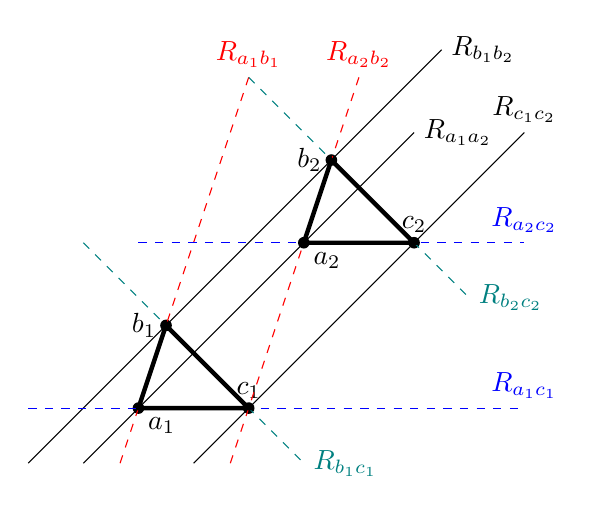
\begin{tikzpicture}[scale=0.7]
                % Los puntos del triángulo 1
                \coordinate (a_1) at (-2,0);
                \coordinate (b_1) at (-1.5,1.5);
                \coordinate (c_1) at (0,0);
    
                % Los puntos del triángulo 2
                \coordinate (a_2) at (1,3);
                \coordinate (b_2) at (3,3);
                \coordinate (c_2) at (1.5,4.5);
    
                % Las rectas que unen los triángulos
                \coordinate (R_a1a2_ini) at (-3,-1);
                \coordinate (R_a1a2_fin) at (3,5);
    
                \coordinate (R_c1c2_ini) at (-1,-1);
                \coordinate (R_c1c2_fin) at (5,5);
    
                \coordinate (R_b1b2_ini) at (-4,-1);
                \coordinate (R_b1b2_fin) at (3.5,6.5);
    
                % Las rectas que unen los vértices del triángulo 1
                \coordinate (R_a1b1_ini) at (-7/3,-1);
                \coordinate (R_a1b1_fin) at (0,6);
    
                \coordinate (R_a1c1_ini) at (-4,0);
                \coordinate (R_a1c1_fin) at (5,0);
    
                \coordinate (R_b1c1_ini) at (-3,3);
                \coordinate (R_b1c1_fin) at (1,-1);
    
                % Las rectas que unen los vértices del triángulo 2
                \coordinate (R_a2b2_ini) at (-1/3,-1);
                \coordinate (R_a2b2_fin) at (2,6);
    
                \coordinate (R_a2c2_ini) at (-2,3);
                \coordinate (R_a2c2_fin) at (5,3);
    
                \coordinate (R_b2c2_ini) at (0,6);
                \coordinate (R_b2c2_fin) at (4,2);
    
                % Dibujamos los puntos del triángulo 1
                \fill (a_1) circle (3pt) node [below right] {$a_1$};
                \fill (b_1) circle (3pt) node [left] {$b_1$};
                \fill (c_1) circle (3pt) node [above] {$c_1$};
    
                % Dibujamos los puntos del triángulo 2
                \fill (a_2) circle (3pt) node [below right] {$a_2$};
                \fill (b_2) circle (3pt) node [above] {$c_2$};
                \fill (c_2) circle (3pt) node [left] {$b_2$};
    
                % Dibujamos las rectas que unen los triángulos
                \draw[] (R_a1a2_ini) -- (R_a1a2_fin) node [right] {$R_{a_1a_2}$};
                \draw[] (R_b1b2_ini) -- (R_b1b2_fin) node [right] {$R_{b_1b_2}$};
                \draw[] (R_c1c2_ini) -- (R_c1c2_fin) node [above] {$R_{c_1c_2}$};
    
                % Dibujamos las rectas que unen los vértices del triángulo 1
                \draw[dashed, red] (R_a1b1_ini) -- (R_a1b1_fin) node [above] {$R_{a_1b_1}$};
                \draw[dashed, blue] (R_a1c1_ini) -- (R_a1c1_fin) node [above] {$R_{a_1c_1}$};
                \draw[dashed, teal] (R_b1c1_ini) -- (R_b1c1_fin) node [right] {$R_{b_1c_1}$};
    
                % Dibujamos las rectas que unen los vértices del triángulo 2
                \draw[dashed, red] (R_a2b2_ini) -- (R_a2b2_fin) node [above] {$R_{a_2b_2}$};
                \draw[dashed, blue] (R_a2c2_ini) -- (R_a2c2_fin) node [above] {$R_{a_2c_2}$};
                \draw[dashed, teal] (R_b2c2_ini) -- (R_b2c2_fin) node [right] {$R_{b_2c_2}$};
    
                % Dibujamos los triángulos
                \draw[ultra thick] (a_1) -- (b_1) -- (c_1) -- cycle;
                \draw[ultra thick] (a_2) -- (b_2) -- (c_2) -- cycle;
            \end{tikzpicture}
            \caption{\centering Rectas paralelas.}
        \end{subfigure}
        \caption{\centering Representación gráfica del Ejercicio \ref{ej:5.1.38}.}
    \end{figure}

    En el caso de que las rectas $R_{a_1a_2}$, $R_{b_1b_2}$ y $R_{c_1c_2}$ sean paralelas,
    consideramos la traslación según el vector $\vec{a_1a_2}$, En el caso de que se corten en el mismo punto $P\in \cc{A}$,
    consideramos la homotecia de centro $P$ que lleva $a_1$ en $a_2$.

    En ambos casos, tenemos que $f(a_1)=a_2$, y como $f$ lleva rectas en rectas paralelas
    y $R_{a_1b_1}\|R_{a_2b_2}$, entonces $f(b_1)=b_2$. Análogamente, $f(c_1)=c_2$.

    Sea ahora $\vec{b_1c_1}\in \vec{R_{b_1c_1}}$. Tenemos que:
    \begin{align*}
        \vec{f}\left(\vec{b_1c_1}\right) &= \lm \vec{b_1c_1} =\\
        &= \vec{f(b_1)f(c_1)} = \vec{b_2c_2}
    \end{align*}
    donde en la primera igualdad he aplicado que $\vec{f}=\lm Id$, con $\lm \in \bb{R}^\ast$,
    y en la segunda igualdad he aplicado la definición de lineal de una aplicación afín.

    Por tanto, tenemos que $\vec{b_1c_1}\in \cc{L}\{\vec{b_2c_2}\}$, es decir, $R_{b_1c_1}\|R_{b_2c_2}$.
\end{ejercicio}



\begin{ejercicio}
    Demuestra que la composición de dos simetrías respecto de dos puntos distintos es una traslación.

    Sea $\cc{A}$ un espacio afín, y sean $p,q \in \cc{A}$ dos puntos distintos. Por el Lema \ref{lema:SimetriaCentral}, tenemos que:
    \begin{equation*}
        \sigma_p \circ \sigma_q = H_{p, -1} \circ H_{q, -1}
    \end{equation*}

    Tenemos por tanto que la composición es afín, y su lineal asociada es:
    \begin{equation*}
        \vec{\sigma_p \circ \sigma_q} = -Id_{\cc{A}} \circ -Id_{\cc{A}} = Id_{\cc{A}}
    \end{equation*}

    Por tanto, por la caracterización de las traslaciones, tenemos que $\sigma_p \circ \sigma_q$ es una traslación.
\end{ejercicio}